% Template for PLoS
% Version 3.4 January 2017
%
% % % % % % % % % % % % % % % % % % % % % %
%
% -- IMPORTANT NOTE
%
% This template contains comments intended
% to minimize problems and delays during our production
% process. Please follow the template instructions
% whenever possible.
%
% % % % % % % % % % % % % % % % % % % % % % %
%
% Once your paper is accepted for publication,
% PLEASE REMOVE ALL TRACKED CHANGES in this file
% and leave only the final text of your manuscript.
% PLOS recommends the use of latexdiff to track changes during review, as this will help to maintain a clean tex file.
% Visit https://www.ctan.org/pkg/latexdiff?lang=en for info or contact us at latex@plos.org.
%
%
% There are no restrictions on package use within the LaTeX files except that
% no packages listed in the template may be deleted.
%
% Please do not include colors or graphics in the text.
%
% The manuscript LaTeX source should be contained within a single file (do not use \input, \externaldocument, or similar commands).
%
% % % % % % % % % % % % % % % % % % % % % % %
%
% -- FIGURES AND TABLES
%
% Please include tables/figure captions directly after the paragraph where they are first cited in the text.
%
% DO NOT INCLUDE GRAPHICS IN YOUR MANUSCRIPT
% - Figures should be uploaded separately from your manuscript file.
% - Figures generated using LaTeX should be extracted and removed from the PDF before submission.
% - Figures containing multiple panels/subfigures must be combined into one image file before submission.
% For figure citations, please use "Fig" instead of "Figure".
% See http://journals.plos.org/plosone/s/figures for PLOS figure guidelines.
%
% Tables should be cell-based and may not contain:
% - spacing/line breaks within cells to alter layout or alignment
% - do not nest tabular environments (no tabular environments within tabular environments)
% - no graphics or colored text (cell background color/shading OK)
% See http://journals.plos.org/plosone/s/tables for table guidelines.
%
% For tables that exceed the width of the text column, use the adjustwidth environment as illustrated in the example table in text below.
%
% % % % % % % % % % % % % % % % % % % % % % % %
%
% -- EQUATIONS, MATH SYMBOLS, SUBSCRIPTS, AND SUPERSCRIPTS
%
% IMPORTANT
% Below are a few tips to help format your equations and other special characters according to our specifications. For more tips to help reduce the possibility of formatting errors during conversion, please see our LaTeX guidelines at http://journals.plos.org/plosone/s/latex
%
% For inline equations, please be sure to include all portions of an equation in the math environment.  For example, x$^2$ is incorrect; this should be formatted as $x^2$ (or $\mathrm{x}^2$ if the romanized font is desired).
%
% Do not include text that is not math in the math environment. For example, CO2 should be written as CO\textsubscript{2} instead of CO$_2$.
%
% Please add line breaks to long display equations when possible in order to fit size of the column.
%
% For inline equations, please do not include punctuation (commas, etc) within the math environment unless this is part of the equation.
%
% When adding superscript or subscripts outside of brackets/braces, please group using {}.  For example, change "[U(D,E,\gamma)]^2" to "{[U(D,E,\gamma)]}^2".
%
% Do not use \cal for caligraphic font.  Instead, use \mathcal{}
%
% % % % % % % % % % % % % % % % % % % % % % % %
%
% Please contact latex@plos.org with any questions.
%
% % % % % % % % % % % % % % % % % % % % % % % %

\documentclass[10pt,letterpaper]{article}
\usepackage[top=0.85in,left=2.75in,footskip=0.75in]{geometry}

% amsmath and amssymb packages, useful for mathematical formulas and symbols
\usepackage{amsmath,amssymb}

% Use adjustwidth environment to exceed column width (see example table in text)
\usepackage{changepage}

% Use Unicode characters when possible
\usepackage[utf8x]{inputenc}

% textcomp package and marvosym package for additional characters
\usepackage{textcomp,marvosym}

% cite package, to clean up citations in the main text. Do not remove.
\usepackage{cite}

% Use nameref to cite supporting information files (see Supporting Information section for more info)
\usepackage{nameref,hyperref}

% line numbers
\usepackage[right]{lineno}

% ligatures disabled
\usepackage{microtype}
\DisableLigatures[f]{encoding = *, family = * }

% color can be used to apply background shading to table cells only
\usepackage[table]{xcolor}

% array package and thick rules for tables
\usepackage{array}

% create "+" rule type for thick vertical lines
\newcolumntype{+}{!{\vrule width 2pt}}

% create \thickcline for thick horizontal lines of variable length
\newlength\savedwidth
\newcommand\thickcline[1]{%
  \noalign{\global\savedwidth\arrayrulewidth\global\arrayrulewidth 2pt}%
  \cline{#1}%
  \noalign{\vskip\arrayrulewidth}%
  \noalign{\global\arrayrulewidth\savedwidth}%
}

% \thickhline command for thick horizontal lines that span the table
\newcommand\thickhline{\noalign{\global\savedwidth\arrayrulewidth\global\arrayrulewidth 2pt}%
\hline
\noalign{\global\arrayrulewidth\savedwidth}}


% Remove comment for double spacing
%\usepackage{setspace}
%\doublespacing

% Text layout
\raggedright
\setlength{\parindent}{0.5cm}
\textwidth 5.25in
\textheight 8.75in

% Bold the 'Figure #' in the caption and separate it from the title/caption with a period
% Captions will be left justified
\usepackage[aboveskip=1pt,labelfont=bf,labelsep=period,justification=raggedright,singlelinecheck=off]{caption}
\renewcommand{\figurename}{Fig}

% Use the PLoS provided BiBTeX style
\bibliographystyle{plos2015}

% Remove brackets from numbering in List of References
\makeatletter
\renewcommand{\@biblabel}[1]{\quad#1.}
\makeatother

% Leave date blank
\date{}

% Header and Footer with logo
\usepackage{lastpage,fancyhdr,graphicx}
\usepackage{epstopdf}
\pagestyle{myheadings}
\pagestyle{fancy}
\fancyhf{}
\setlength{\headheight}{27.023pt}
\lhead{
\includegraphics[width=2.0in]{PLOS-submission.eps}}
\rfoot{\thepage/\pageref{LastPage}}
\renewcommand{\footrule}{\hrule height 2pt \vspace{2mm}}
\fancyheadoffset[L]{2.25in}
\fancyfootoffset[L]{2.25in}
\lfoot{\sf PLOS}

%% END MACROS SECTION
\usepackage{makecell}
\usepackage{multirow}
\usepackage{booktabs}




\begin{document}

\vspace*{0.2in}

% Title must be 250 characters or less.
\begin{flushleft}
{\Large
\textbf\newline{The evolution of evolvability: Changing environments promote rapid adaptation in digital organisms} % Please use "sentence case" for title and headings (capitalize only the first word in a title (or heading), the first word in a subtitle (or subheading), and any proper nouns).
}
\newline
\\
Rosangela Canino-Koning\textsuperscript{1,2*},
Michael J. Wiser\textsuperscript{2,3},
Charles Ofria\textsuperscript{1,2,3\ddag}
\\
\bigskip
\textbf{1} Department of Computer Science and Engineering, Michigan State University, East Lansing, MI, USA
\\
\textbf{2} BEACON Center for the Study of Evolution in Action, Michigan State University, East Lansing, MI, USA
\\
\textbf{3} Ecology, Evolutionary Biology, and Behavior, Michigan State University, East Lansing, MI, USA
\\
\bigskip

% Additional Equal Contribution Note
% Also use this double-dagger symbol for special authorship notes, such as senior authorship.
\ddag These authors also contributed equally to this work.

% Use the asterisk to denote corresponding authorship and provide email address in note below.
* caninoko@msu.edu

\end{flushleft}
% Please keep the abstract below 300 words
\section*{Abstract}
Genetic spaces are often described in terms of fitness landscapes or genotype-to-phenotype maps, where each potential genetic sequence is associated with its phenotypic properties and is linked to other genotypes that are a single mutational step away.  The positions close to a genotype make up its "mutational landscape" and, in aggregate, determine the short-term evolutionary potential of a population.
% @CAO: The first part of this paragraph is providing terminology.  The rest is, I assume, talking about the contributions of this paper, but we never make that clear (a casual reader might assume that we're still providing background.)  If the impact of more phenotypes in a neighborhood is all well accepted already, ignore this comment.
Populations with wider ranges of phenotypes in their mutational neighborhood tend to be more evolvable. Likewise, those with fewer phenotypic changes available in their local neighborhoods are more mutationally robust. As such, forces that alter the distribution of phenotypes available by mutation can have a profound effect on subsequent evolutionary dynamics.

Environmental change alters a fitness landscape and is believed to create selective pressures for populations to rapidly adapt to those changes.  Indeed, we demonstrate that cyclically-changing environments can push populations toward more evolvable mutational landscapes where a wide range of alternate phenotypes are available, though purely deleterious mutations remain suppressed. We further show that populations in environments with drastic changes change phenotypes more readily than those in environments with more benign changes. We trace this effect to repeated population bottlenecks in the harsh environments, which result in shorter coalescence times and keep populations in regions of the mutational landscape where the phenotypic shifts in question are more likely to occur.

\linenumbers

% Use "Eq" instead of "Equation" for equation citations.
\section*{Introduction}
%=fitness landscapes are useful math but real-world landscapes are more complex than theory
Fitness landscapes are a mathematical tool to map genetic sequences to expected evolutionary fitness. Many studies have examined the important role that different types of fitness landscapes play on evolutionary dynamics and outcomes, both in biological populations \cite{khan_negative_2011,szendro_quantitative_2013,weinreich_darwinian_2006,nahum_tortoisehare_2015} and in evolutionary computation settings \cite{merz_fitness_2000,humeau_paradiseo-mo:_2013,kallel_theoretical_2013}. However, real-world fitness landscapes are far more complex and varied than the limited or idealized models that are used in most of these studies. Neighboring regions of real landscapes can have starkly different properties from each other based on the effects of and interactions among mutations (i.e., the mutational landscape).  

%=properties of landscapes depend on architecture
Examples of the type of properties that we are interested in include robustness, epistasis, and modularity, all of which are measurements of how information is organized inside of a genome and commonly categorized as components of an organism's ``genetic architecture''. Isolated pockets in a landscape can often be characteristically different from the landscape as a whole due to the amount and organization of genetic information.  In fact, in most natural fitness landscapes, the vast majority of neighborhoods consist entirely of non-replicating genomes with zero fitness (and thus no genetic information), making life itself appear to be a rare exception \cite{gavrilets_fitness_2004}.

%=evolution is limited to viable areas
Evolution on these convoluted landscapes is clearly limited to those regions that have non-zero fitness, with a selective pressure for fitness to increase. Beyond that, however, populations can evolve toward neighborhoods with specific local properties based on the evolutionary forces acting upon the populations.  For example, high mutation rates drive populations toward neighborhoods with a higher fraction of neutral mutations in an effect dubbed “survival of the flattest” \cite{wilke_evolution_2001}. Similarly, sexual populations tend toward regions of the fitness landscape with more modularity \cite{misevic_sexual_2006} and more negative epistasis \cite{misevic_experiments_2010} than otherwise equivalent asexual populations.

%=understanding dynamics is of broad interest
Understanding these dynamics is of broad interest.  It is important to evolutionary computation, given the strong influence of local landscape properties on the quality of the final solutions that an evolving population is able to obtain. Its relevance to evolutionary biology is equally obvious -- the local landscape that a population occupies will influence the selective forces at play in the population, creating a feedback cycle between these two important evolutionary factors \cite{zaman_coevolution_2014,meyer_repeatability_2012}. Disentangling such interactions is likely to provide further insights into fundamental evolutionary dynamics.  Computational artificial life systems have the advantage of being able to bridge these two realms: they have unconstrained evolutionary dynamics similar to natural systems, while maintaining the ability to rapidly perform experiments and collect any data we need about populations or their local landscapes.
% * <mjwiser@gmail.com> 2016-12-01T20:34:49.014Z:
%
% I can suggest other citations here, so we're not solely citing people out of Charles' and Rich's labs.
%
% ^ <mjwiser@gmail.com> 2017-01-30T18:26:00.719Z:
%
% A few suggested citations here, given Charles' agreement:
% Aita et al 2002.  Surveying a local fitness landscape of a protein with epistatic sites for the study of directed evolution
% Bershtein et al 2006 Robustness–epistasis link shapes the fitness landscape of a randomly drifting protein
% Martin and Lenormand 2006 THE FITNESS EFFECT OF MUTATIONS ACROSS ENVIRONMENTS: A SURVEY IN LIGHT OF FITNESS LANDSCAPE MODELS
% Kvitek and Sherlock 2009 Reciprocal Sign Epistasis between Frequently Experimentally Evolved Adaptive Mutations Causes a Rugged Fitness Landscape
%
% ^ <mjwiser@gmail.com> 2017-01-30T18:26:30.874Z:
%
% I can pick out a few more recent ones if these seem older than you'd prefer.
%
% ^.
% @CAO: Good call Mike!

\subsection*{Evolvability and Genetic Architecture}
%=what is evolvability, to us
Evolvability refers to a series of distinct but overlapping concepts that are generally concerned with adaptation, variation, and/or novelty generation \cite{pigliucci_is_2008}. Depending on your perspective, evolvability can describe the response to selection at the population level\cite{fisher_genetical_1930,houle_comparing_1992}, the ability of populations to adapt to changing conditions\cite{belle_code_2002}, larger phenomena such as variability generation\cite{gunter_p._wagner_perspective:_1996}, 
exploration of neutral spaces and robustness\cite{andreas_wagner_robustness_2005,kitano_biological_2004}, 
generation of novel features\cite{alberch_genes_1991,brookfield_evolution:_2001}, 
or even the potential to generate clade-level innovations\cite{kirschner_evolvability_1998} 
and major transitions\cite{smith_major_1995}. For the purposes this paper, we will focus on evolvability as the capability of genomes to generate adaptive variation in response to mutation. 

%=how it affects short term evo
In the short-term, this kind of evolvability determines a population's response to selection. This kind of evolvability depends primarily on the organization and interrelation of information in the genome; that is, the genetic architecture, and the resulting genotype-to-phenotype map \cite{gunter_p._wagner_perspective:_1996}. An example of evolvable architecture can be found in some bacterial genomes that contain highly mutable genome regions, called contingency loci. Small sets of insertions or deletions to these regions create transcription frameshifts that alter the expression of nearby coding regions, thus allowing populations to easily switch phenotypes via minor mutations. Contingency loci are most often seen in the genomes of pathogens, which are subject to frequent environmental shifts caused by the host immune system \cite{bayliss_simple_2001}. Thus, these populations are able to produce large amounts of heritable variation despite the reduction in population diversity resulting from population bottlenecks.

%=how it affects long-term evo
For longer timescales, evolvability is concerned more with variability generation and exploration of neutral spaces. Populations that exhibit this kind of evolvability would possess genomes with genetic architectures that more easily traverse the mutational landscape along neutral roads and thereby discover new fitness peaks while avoiding crossing fitness valleys. This kind of evolvability would allow populations to more easily colonize new ecological niches and form new clades\cite{kirschner_evolvability_1998,brookfield_evolution:_2001}.

%=connection between short/long term evo non-obvious
Despite some common features, the relationship between short-term and long-term evolvability is not obvious. Architectural features and evolutionary pressures that might convey short-term evolvability may not be the same as those that confer longer-term evolvability\cite{pigliucci_is_2008}. For example, features that promote rapid adaptation to a harsh fluctuating environment might reduce fitness in constant or benign fluctuating environments as compared to that of wild-type invaders. Alternately, the adaptation to harsh fluctuating environments and the resulting bottlenecks would potentially reduce diversity to the point where large amounts of neutral novelty generation could not occur.

\subsubsection*{Mutational Landscapes}
%=how mutational landscapes relate
Properties of genetic architectures such as evolvability and robustness are determined by the shape of the resulting mutational landscape \cite{andreas_wagner_robustness_2008}. Robust genetic architectures that can tolerate more mutations without altering their phenotype reside in mutational landscapes that connect to more neutral mutants. Similarly, architectures that more easily switch phenotypes in response to mutation without substantial reduction in fitness, reside in more evolvable regions of genotype-space.

%=not all regions equally accessible
It is worth noting that not all regions of the mutational landscape are equally accessible. Some genome regions may be more resistant to mutation than others \cite{lee_rate_2012}, thereby altering [\@RCK TODO] the probabilities of mutations occurring that lead into certain regions of the mutational landscape. This kind of differential probability may therefore moderate a population's diffusion through the mutational landscape.

% @CAO: How would it be altered?  I'm not sure I understand the last couple of sentences here...
% * <mjwiser@gmail.com> 2017-01-30T18:58:49.934Z:
%
% There are several ways I could interpret this sentence about the Lee paper, so I feel I need to read the paper.  Is it that there are certain regions of a genome that are harder to mutate, either because they are physically constrained or that they are more easily error-checked?  Is it that certain regions of the mutational landscape are more resistant to mutations?  If it's the latter, perhaps a rephrasing along the line of "Some regions of the mutational landscape are more resistant to mutations (preferably with some explanation of how).  As such, regions of the mutational landscape that are bordered by such mutation-resistant regions are less accessible, as the set of genotypes that are mutationally close to them are themselves resistant to mutations."
%
% ^.
% @RCK: Will look into it and clarify.
%=response to selection may be weaker/stronger
Further, response to selection is likely to be weaker in regions of the landscape where there are fewer available mutations that provide potentially adaptive traits, whereas response to selection will be stronger in regions where there are many adaptive variants available within a few mutational steps \cite{alberch_genes_1991,carter_role_2005}. This differential response to selection therefore constrains the ability of populations to diffuse across a fitness landscape.

\subsubsection*{Landscape Metrics}
%=assessing mutational landscapes: D_g
Assessing the qualities of the nearby mutational landscape requires measures that can relate phenotypes and their fitness effects with the probabilities that these mutants will arise in the population. In order to assess the relative neutrality of the nearby mutational network, we will measure the \textbf{Genomic Diffusion Rate} $D_g$ \cite{ofria_evolution_2002}. This rate approximates the overall rate at which the population encounters new neutral genotypes.
%=how to calculate D_g
To calculate the \textbf{Genomic Diffusion Rate} ($D_g$) in the local neighborhood of a genotype, first calculate its \textit{Fidelity} ($F$), or the probability of an offspring sharing this genotype with its parent, by measuring the probability that a single locus is not mutated ($1-\mu)$ and raising it to the power of the genome length ($l$). Next, measure the proportion of 1-step mutants that are neutral or beneficial when compared to the parent ($p_\nu$) as well as those that are detrimental or lethal ($p_d$), which must sum to one ($p_\nu + p_d = 1$).  The \textit{Neutral Fidelity} ($F_\nu$) of a genotype is thus the probability that no harmful mutations occur, assuming no epistasis. Finally, subtracting Fidelity from Neutral Fidelity will yield the overall probability of producing an neutral offspring with a different genotype, yet neutral or better fitness ($D_g$).

\begin{eqnarray}
\label{eq:fidelity}
	F = (1 - \mu)^l
\end{eqnarray}
\begin{eqnarray}
\label{eq:neutral_fidelity}
	F_\nu = (1 - \mu p_d)^l
\end{eqnarray}
\begin{eqnarray}
\label{eq:genomic_diffusion_rate}
	D_g = F_\nu - F
\end{eqnarray}

%=measuring more than neutral exploration. Calculating D_p
Measures of neutral exploration, however, only show part of the picture. While some form of neutrality is necessary for exploring a fitness landscape, new phenotypes must be discovered to achieve higher local evolvability. In order to assess evolvability more specifically, we introduce a related measure, the \textbf{Phenotypic Diffusion Rate} ($D_p$), which represents the probability that an offspring will be fitness-neutral, but also express a different phenotype than its parent. To do so, we must first measure the proportion of one-step mutants that are \textit{phenotypically} neutral as compared to their parent ($p_{p\nu}$) and follow a similar procedure as above, first calculating the probability that a phenotype-changing mutation will occur ($\mu_{pheno}$), then the phenotypic-level fidelity ($F_{p\nu}$).
\begin{eqnarray}
\label{eq:phenotypic_mutation_rate}
	\mu_{pheno} = \mu (1- p_{p\nu})
\end{eqnarray}
\begin{eqnarray}
\label{eq:phenotypic_fidelity}
	F_{p\nu} = (1 - \mu_{pheno})^l
\end{eqnarray}
\begin{eqnarray}
\label{eq:phenotypic_diffusion_rate}
	D_p = F_\nu - F_{p\nu}
\end{eqnarray}
The difference between the overall neutral fidelity and the phenotype-preserving neutral fidelity ($F_\nu - F_{p\nu}$) yields the phenotypic diffusion rate.

\subsubsection*{Expected Value of Fitness Landscapes}
%=addressing expected fitness in fluctuating environments
In the context of changing environments, the expected fitness value ($E(w)$), and thus the neutrality, of a mutant in the mutational landscape will vary depending on the environmental context. So, in one environment, a mutant may be highly fit, but the same allele may be highly deleterious in a different environment. In order to address this variation, all metrics must be normalized by the probability that a particular environment will occur ($P_i$). That is, the nearby mutational landscape must be evaluated in each possible environment, yielding a traditional fitness landscape. Then, the set of fitnesses of each mutant ($w_i$) in each environment must be aggregated according to the probability of that environment occurring.
\begin{eqnarray}
\label{eq:expected_fitness_value}
	E(w) = \displaystyle\sum_{i=1}^{e} w_i P_i
\end{eqnarray}

\subsection*{Changing environments create more paths to different kinds of phenotypes}
%=sustained directional selection for adaptation
Sustained directional selection adjusts the composition of phenotypes and genotypes in a population \cite{wright_evolution_1931}, typically moving that population across the mutational landscape to local regions of higher fitness. When populations find a fitness peak, they tend to cluster there, and exploration of that region of the landscape slows dramatically.

%=CE promotes exploration
In changing environments, however, the direction of selection is not fixed and peaks are not stable.  Instead, as the environment changes, populations are driven to explore new regions of the mutational landscape \cite{kashtan_varying_2007,connelly_negative_2015}. As they proceed, populations accumulate and carry with the genetic material acquired in prior explorations and adaptations, and use this history as raw material for new adaptation \cite{mcclintock_significance_1993}. Indeed, earlier work has shown that changing environments promote evolvability in many contexts, without compromising robustness \cite{crombach_evolution_2008,wilke_evolution_2001}. Strength of selection is also an important component of this exploration, since the harshness of the environment drives the speed with which organisms adapt to new conditions \cite{goddard_sex_2005}.

%=CE not only drives exploration, but changes surrounding mutational landscape environment
In this paper, we show how changing environments not only drive exploration of the mutational landscape, but also select for populations whose genetic architectures are qualitatively different than those from populations evolved in static environmental conditions. In particular, we show that populations evolved under harsh, cyclically-changing environments have many more changes along their phylogenetic histories than those evolved in static or benign changing environments. Organisms evolved in these populations also contain reservoirs of pseudogene-like vestigial loci that were acquired and deactivated through repeated adaptation and fixation cycles. As a result, populations evolved in these harsh cyclically-changing environments are low in standing neutral diversity at the population level, but they still connect locally with many more phenotypically-interesting regions of the mutational landscape than more diverse populations evolved in static or benign environments.

\section*{Methods}

\subsection*{Digital Evolution}
%=DE for studying evolution
Digital Evolution uses self-replicating computer programs as model organisms to study evolutionary dynamics~\cite{mckinley_harnessing_2008}. Unlike theoretical simulations, digital organisms have a fully functional genome that direct them to self-replicate, mutate, and compete with their peers for resources and space in which to reproduce. Because digital organisms undergo genetic mutations (i.e., variation) that are passed on to their offspring (inheritance), and their survival is based on the actions they take (differential selection), they undergo evolution by natural selection. % @CAO Cite Dennett?

%=DE is better than natural for three reasons. 1 - reproduction rate
Digital organisms do not suffer from many of the drawbacks of experimentation on natural organisms.  Three of the advantages of digital organisms are particularly relevant for our study.  First, the rates of reproduction in digital systems are much faster than in even the most rapidly-reproducing physical organisms; we can process generations of organisms in seconds, rather than the hours required for the fastest biological organisms under sustained conditions \cite{ryan_evolution_1953,lenski_long-term_1991}, or the weeks to years needed for more complex multicellular organisms \cite{anderson_outcrossing_2010,stearns_experimental_2000}.

%=2 - DE is more controllable
Second, using digital organisms allows us to tightly control and verify experimental conditions. For example, in physical organisms, factors such as mutation rate can generally be measured only after the fact, or coarsely altered through mutagens. In digital organisms, however, we can not only control mutation rates with fine-grained precision, but also types and probabilities of different types mutations (e.g., substitutions vs. insertions vs. deletions). Furthermore, we are also able to track and replay the evolutionary history of every organism at any point in time to verify that unusual or unexpected results do not represent measurement error.  This ability to exactly replicate evolutionary results at an individual organism level is firmly out of reach for experiments with physical organisms.

%=3 - DE is completely knowable
Finally, we can precisely and perfectly map the mutational landscape around the genome of a digital organism, and identify the role of every site in its genome\cite{ofria_evolution_2002}; such exhaustive techniques are not feasible in even the simplest physical organisms.  All of these factors make digital organisms ideal for studying the effects of changing environments on the mutational landscape.

\subsubsection*{Avida Digital Evolution Platform}
%=Avida for doing these experiments
We used Avida \cite{lenski_evolutionary_2003} to examine the effects of cyclic changing environments on the genomes of evolved digital organisms. Avida is a software platform for performing evolution experiments with digital organisms in a virtual world.

%=[FIGURE - Avida CPU]
\begin{figure}[!h]
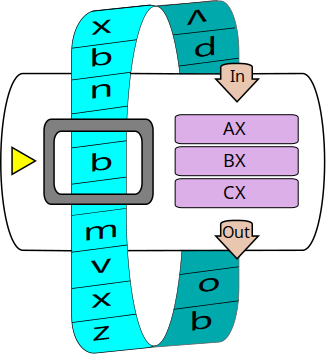
\includegraphics[width=0.5\columnwidth]{figures/squishedCPU_extra.png}
\caption{{\bf An example virtual CPU from Avida}, with a circular genome (blue), three registers (purple), input and output handlers (tan), and an instruction pointer (yellow) indicating the next instruction to be executed.%
}\label{fig:cpu}
\end{figure}

%=description of Avida organism
An Avida organism is composed of a circular genome of assembly-like computer instructions that are executed in a virtual CPU (Fig~\ref{fig:cpu}). Populations of these organisms are placed in a toroidal world in individual cells where they are allowed to execute, reproduce, compete for space, mutate, and evolve.

% @CAO: I feel like a lot of this paragraph repeats information from the last section that was more generically about digital evolution.  We should probably tighten it up here.
%=Avida are self-replicating, but without perfect fidelity
Organisms in Avida are self-replicating, and experience mutation. The genome in the initial default organism contains all of the instructions necessary for reproduction. However, the instructions are not copied into an offspring with perfect fidelity. By default, the reproductive copy instruction is faulty, meaning that it will probabilistically introduce errors (mutations) into the offspring genomes. These offspring organisms execute their own genomes even when different from their parent, and in turn pass on their inherited mutations, along with new mutations, to their own offspring (i.e., variation in the systems is heritable).

%=Avida worlds are constrained and thus competition
Avida worlds can be space- or resource-constrained. Avida allows the experimenter to configure many aspects of the environment, thus subjecting the organisms to various kinds of selective pressures.  In many cases, these environments will include resources that can be metabolized by performing specific functions or activities, resulting in a boost to execution speed that gives the organisms a competitive advantage. However, even without explicit external pressures, organisms still experience an implicit pressure to execute more quickly and efficiently. The organisms that run fastest are typically able to also reproduce fastest, and thus out-compete their peers for space.

%=Avida and paper download information
%=[TODO - make the new git repos for the journal paper]
Avida is available for download without cost from \url{http://avida.devosoft.org/}, and specific versions along with data-files to reproduce the experiments described in this paper may be found at \url{https://github.com/voidptr/avida} and \url{https://github.com/voidptr/ce_evolvability}.

\subsection*{Experimental Design}
%=design for experimental environment (CCE vs SCE, and short vs long)
In order to examine the dynamics and mechanisms of evolving populations in changing environments, we performed two sets of experiments (cyclic vs stochastic changing environments), each divided into two phases (short-term evolvability vs. long-term evolvability). The cyclic environments are designed to simulate predictable cycles of change, such as day/night or seasonal cycles, whereas the stochastic environments represents less predictable oscillations in environmental states, such as random weather patterns, or climactic changes. The first phase of each set of experiments allows organisms to adapt to a predictable set of environments, whereas the second phase introduces the change-evolved populations to a completely new environment. Thus, the first phase explores short-term evolvability dynamics, and the second phase addresses the relationship between short-term and long-term evolvability. See Table~\ref{treatments}

%\begin{table}[!ht]
%\begin{adjustwidth}{-2.25in}{0in} % Comment out/remove adjustwidth environment if table fits in text column.
%\centering
%\caption{
%{\bf Experimental Treatments}}
%\begin{tabular}{|l+l|l|l|l|l|l|}
%\hline
%{\bf Treatment} & {\bf Change Type} & {\bf Harshness} & {\bf Phase 2}\\ \thickline
%\multicolumn{1}{|l|}{\bf Treatment} & \multicolumn{3}{|l|}{\bf Phase 1} & \multicolumn{2}{|l|}{\bf Phase 2}	\\ \hline
%			& {\bf Cycle} 	& {\bf Harshness} & {\bf Tasks Rewarded} 							&	 	& 	\\ \hline
%Control		&n/a			&n/a		& XOR and EQU (constant) 								&No CE 	& XOR, EQU, Logic-77 (constant) \\ \hline
%CCE-Benign	&Cyclic			&Benign 	& \makecell{XOR (constant) \\ EQU (fluctuating 0/+)}	&No CE 	& XOR, EQU, Logic-77 (constant) \\
%			&				&			& 														&CE		\\ \hline
%CCE-Harsh	&				&Harsh		& \makecell{XOR (constant) \\ EQU (fluctuating -/+)}	&No CE	\\
%			&				&			& 														&CE		\\ \hline
%SCE-Benign	&Stochastic		&Benign		& \makecell{XOR (constant) \\ EQU (fluctuating 0/+)}	&No CE	\\
%			&				&			& 														&CE		\\ \hline
%SCE-Harsh	&				&Harsh		& \makecell{XOR (constant) \\ EQU (fluctuating -/+)}	&No CE	\\
%			&				&			& 														&CE		\\ \hline
%\end{tabular}
%\begin{flushleft} Experimental treatments. Four types of cyclic changing environment. Each is split into two treatments for phase two, one continuing with the changing environment, and one without. [\@RCK TODO - Tidy up this table]
%\end{flushleft}
%\label{treatments}
%\end{adjustwidth}
%\end{table}

\begin{table}[]
\centering
\caption{{\bf Experimental Treatments}}
\label{my-label}
\begin{tabular}{|l|l|l|l|l|l|}
\hline
\multicolumn{2}{|c|}{\multirow{2}{*}{\textbf{\begin{tabular}[c]{@{}c@{}}Treatment\\ Name\end{tabular}}}} & \multicolumn{1}{c|}{\multirow{2}{*}{\textbf{Cycle}}}                     & \multicolumn{1}{c|}{\textbf{Phase 1}}                                                     & \multicolumn{2}{c|}{\textbf{Phase 2}}                                                                                                 \\ \cline{4-6} 
\multicolumn{2}{|c|}{}                                                                                   & \multicolumn{1}{c|}{}                                                    & \multicolumn{1}{c|}{\textbf{Tasks}}                                                       & \multicolumn{1}{c|}{\textbf{Tasks}}                                                            & \multicolumn{1}{c|}{\textbf{Cycle?}} \\ \hline
%row1
\multicolumn{2}{|l|}{Control}                                                                          & \multicolumn{1}{l|}{n/a}                                                                      & \multicolumn{1}{l|}{\begin{tabular}[c]{@{}l@{}}XOR and EQU \\ (constant)\end{tabular}}                         & \multicolumn{1}{l|}{\begin{tabular}[c]{@{}l@{}}XOR and EQU \\ (constant)\end{tabular}}                              & \multicolumn{1}{l|}{N}               \\ \midrule
%row2
\multirow{2}{*}{CCE-Benign}                                      & A                                     & \multirow{2}{*}{\begin{tabular}[c]{@{}l@{}}Cyclic\\ Benign\end{tabular}} & \multirow{2}{*}{\begin{tabular}[c]{@{}l@{}}XOR (constant)\\ EQU (fluct 0/+)\end{tabular}} & \begin{tabular}[c]{@{}l@{}}XOR (constant)\\ EQU (fluct 0/+)\\ Logic 77 (constant)\end{tabular} & Y                                    \\ \cline{2-2} \cline{5-6} 
                                                                 & B                                     &                                                                          &                                                                                           & \begin{tabular}[c]{@{}l@{}}XOR (constant)\\ EQU (constant)\\ Logic-77 (constant)\end{tabular}  & N                                    \\ \hline
%row3
\multirow{2}{*}{CCE-Harsh}                                      & A                                     & \multirow{2}{*}{\begin{tabular}[c]{@{}l@{}}Cyclic\\ Harsh\end{tabular}} & \multirow{2}{*}{\begin{tabular}[c]{@{}l@{}}XOR (constant)\\ EQU (fluct -/+)\end{tabular}} & \begin{tabular}[c]{@{}l@{}}XOR (constant)\\ EQU (fluct -/+)\\ Logic 77 (constant)\end{tabular} & Y                                    \\ \cline{2-2} \cline{5-6} 
                                                                 & B                                     &                                                                          &                                                                                           & \begin{tabular}[c]{@{}l@{}}XOR (constant)\\ EQU (constant)\\ Logic-77 (constant)\end{tabular}  & N                                    \\ \hline
%row4
\multirow{2}{*}{SCE-Benign}                                      & A                                     & \multirow{2}{*}{\begin{tabular}[c]{@{}l@{}}Stochastic\\ Benign\end{tabular}} & \multirow{2}{*}{\begin{tabular}[c]{@{}l@{}}XOR (constant)\\ EQU (fluct 0/+)\end{tabular}} & \begin{tabular}[c]{@{}l@{}}XOR (constant)\\ EQU (fluct 0/+)\\ Logic 77 (constant)\end{tabular} & Y                                    \\ \cline{2-2} \cline{5-6} 
                                                                 & B                                     &                                                                          &                                                                                           & \begin{tabular}[c]{@{}l@{}}XOR (constant)\\ EQU (constant)\\ Logic-77 (constant)\end{tabular}  & N                                    \\ \hline
%row5
\multirow{2}{*}{SCE-Harsh}                                      & A                                     & \multirow{2}{*}{\begin{tabular}[c]{@{}l@{}}Stochastic\\ Harsh\end{tabular}} & \multirow{2}{*}{\begin{tabular}[c]{@{}l@{}}XOR (constant)\\ EQU (fluct -/+)\end{tabular}} & \begin{tabular}[c]{@{}l@{}}XOR (constant)\\ EQU (fluct -/+)\\ Logic 77 (constant)\end{tabular} & Y                                    \\ \cline{2-2} \cline{5-6} 
                                                                 & B                                     &                                                                          &                                                                                           & \begin{tabular}[c]{@{}l@{}}XOR (constant)\\ EQU (constant)\\ Logic-77 (constant)\end{tabular}  & N                                    \\ \hline
                                                                 
\end{tabular}
\begin{flushleft} Experimental treatments. Four types of cyclic changing environment. Each is split into two treatments for phase two, one continuing with the changing environment, and one without. [\@RCK TODO - Tidy up this table]
\end{flushleft}
\label{treatments}
\end{table}


\subsubsection*{Cyclic and Stochastic Changing Environments}
%=explanation of the changing environment treatments - cyclic
For the cyclic environment, we subjected a total of 150 replicate populations of digital organisms to two different treatments of two-phase cyclically changing environments, plus a static control. The environment cycles between equal-length periods of reward and punishment. Each cycle extends for 1000 updates, or roughly 30 generations. In the static control, there is no cycle. Rather, the rewards remain constant. The first phase of the experiment extends for 200 cycles, or 200,000 updates, approximately 6,000 generations.

%=stochastic
The stochastic changing environment experiment is similar to the cyclic environment, except that rather than the environment toggling every 500 updates, the environmental switch happens randomly, with a 0.002 probability of changing on every update. This averages, in the long term, to approximately one switch every 500 updates, but in the short term, the environmental switches are unpredictable.

%=tasks
In phase 1, we set up the system to detect organisms that performed XOR or EQU, two challenging bit-wise logical tasks. In the static control, XOR is rewarded with a CPU speed (and thus fitness) multiple of 8, while EQU is rewarded with a CPU speed multiple of 32. In the harsh treatment, as the cycle progresses, the XOR reward remains constant, while the EQU reward cycles between a 32-fold bonus and a correspondingly harsh 32-fold penalty (i.e., CPU speed is divided by 32 when EQU is performed in the off cycle). The benign treatment is nearly identical to the harsh treatment, except that the reward merely goes away in the off-cycle as opposed to incurring a severe penalty.

%=differences between tasks
In both environments, we identify EQU as the \textit{Fluctuating Task}. XOR, because it is rewarded continuously, is the \textit{Backbone Task}, and is used as a background for comparing the separation or intertwining of functional genetic components in the evolution of EQU. Further, the 4-fold difference in reward level between XOR and EQU encourages the evolution and maintenance of EQU when possible.

%=long term evolvability - new task
The second phase of the experiment continues the evolution of these populations, but introduces them to an entirely new set of rewarded bit-wise logical tasks: the Logic-77 environment. These new tasks use three bit-wise inputs rather than two, and are each rewarded with a constant 1.2-fold bonus to execution. This provides a mild selective pressure to evolve these task, but the benefits to performing them do not overwhelm the existing selective pressure to continue performing XOR or EQU.

%=the organisms
For all of the experiments described in this section, we held the individual genomes at a fixed length of 121\footnote{As part of our initial controls, we hand-wrote an organism with separated sections that performed XOR and EQU. This hand-written organism had 121 instructions and as such we used this genome length as a constraint for the evolve organisms as well.} instructions, but tested the new genomes for mutations after each successful replication event at a substitution probability of 0.00075 per site. We configured the Avida world to have local interactions on a toroidal grid that is 60-by-60 cells (3600 cells in total), and we seeded the initial populations with an ancestor that was previously evolved to perform XOR and EQU under a static reward. The genetic architecture for performing XOR and EQU is tightly intertwined in this ancestral organism, as it was evolved with no selective pressure for modularity.


\section*{Results and Discussion}
%=summary - we found that CE evolved populations are genetically distinct. Stochastic pretty similar to CCE
Our experiments demonstrate that digital organisms that were evolved in changing environments differ substantially from those evolved in static environments in a number of ways. These differences include the number of mutations that fix in the lineage from the ancestor (the ``phylogenetic depth"), key metrics of their genetic architecture, and the presence of reservoirs of pseudogenes that change the nearby mutational landscape. These features represent adaptation to the larger regime of repeated environmental switching. We also show that while populations evolved in cyclic environments are slightly better adapted to change than those evolved in stochastic environments, in most measures of adaptation and short-term evolvability, these differences are generally not significant. This indicates that while regular periodicity may offer a slight advantage for adaptation, stochastic environments perform similarly in most respects. 

\subsection*{Cyclic Changing Environments}

\subsubsection*{Evolutionary History and Population Structure}
%=more phylogenetic depth
Evolution in the harsh cyclic changing environment resulted in populations with substantially higher phylogenetic depth as compared to those evolved in static or benign environments. At each environmental shift, adaptive mutations rapidly swept and fixed in the populations. (Fig~\ref{fig:flamegraph})

%=[FIGURE - flamegraph]
\begin{figure}[!h]
%\begin{center}
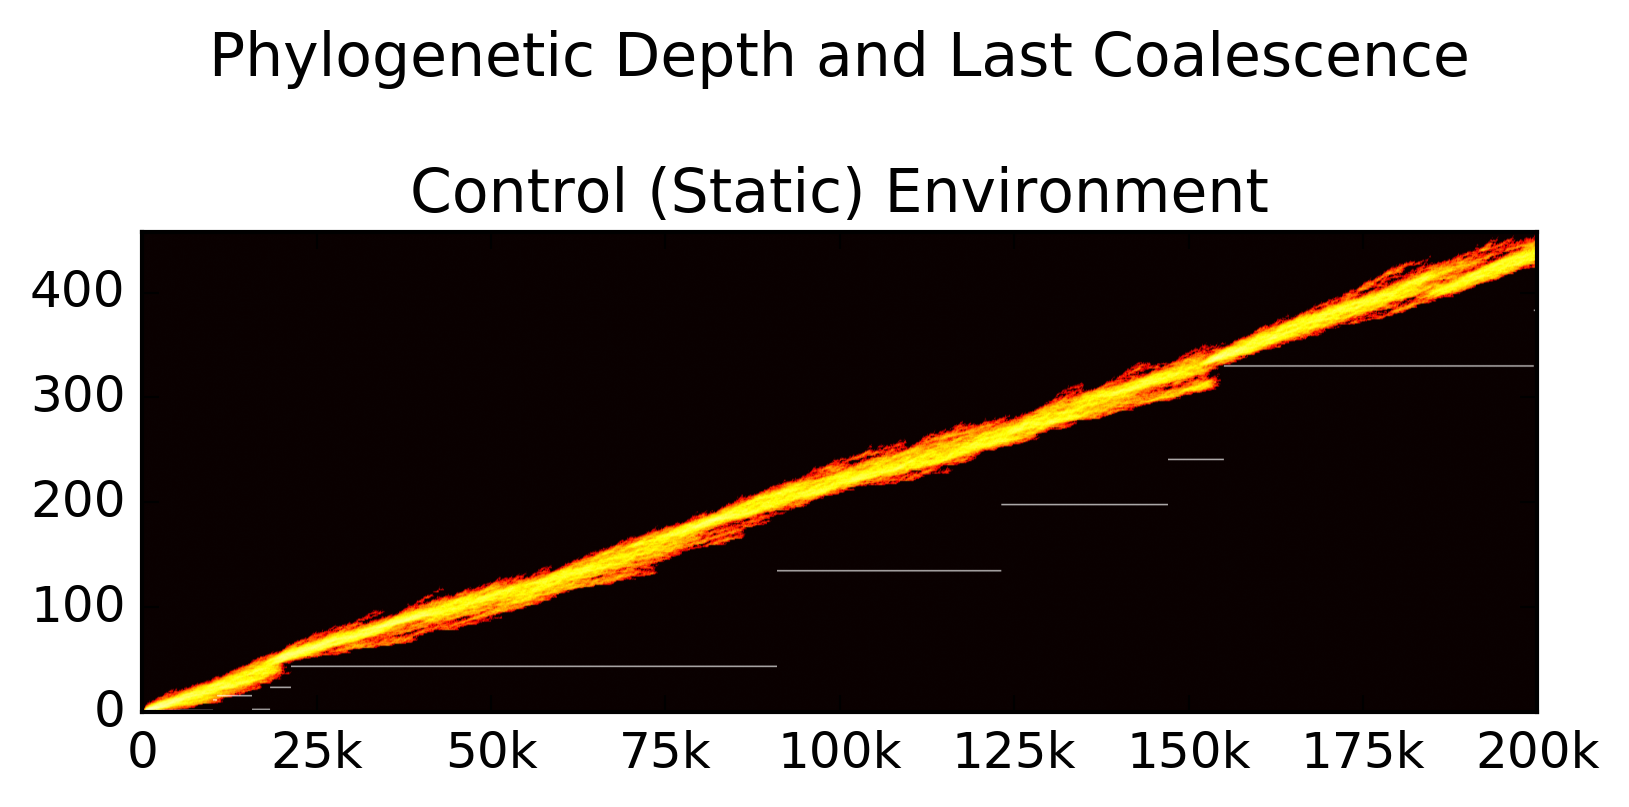
\includegraphics[trim={-0.88cm 0 0.25cm 0},clip,width=1\columnwidth]{figures/control__phylodepth_with_coalescense.png}
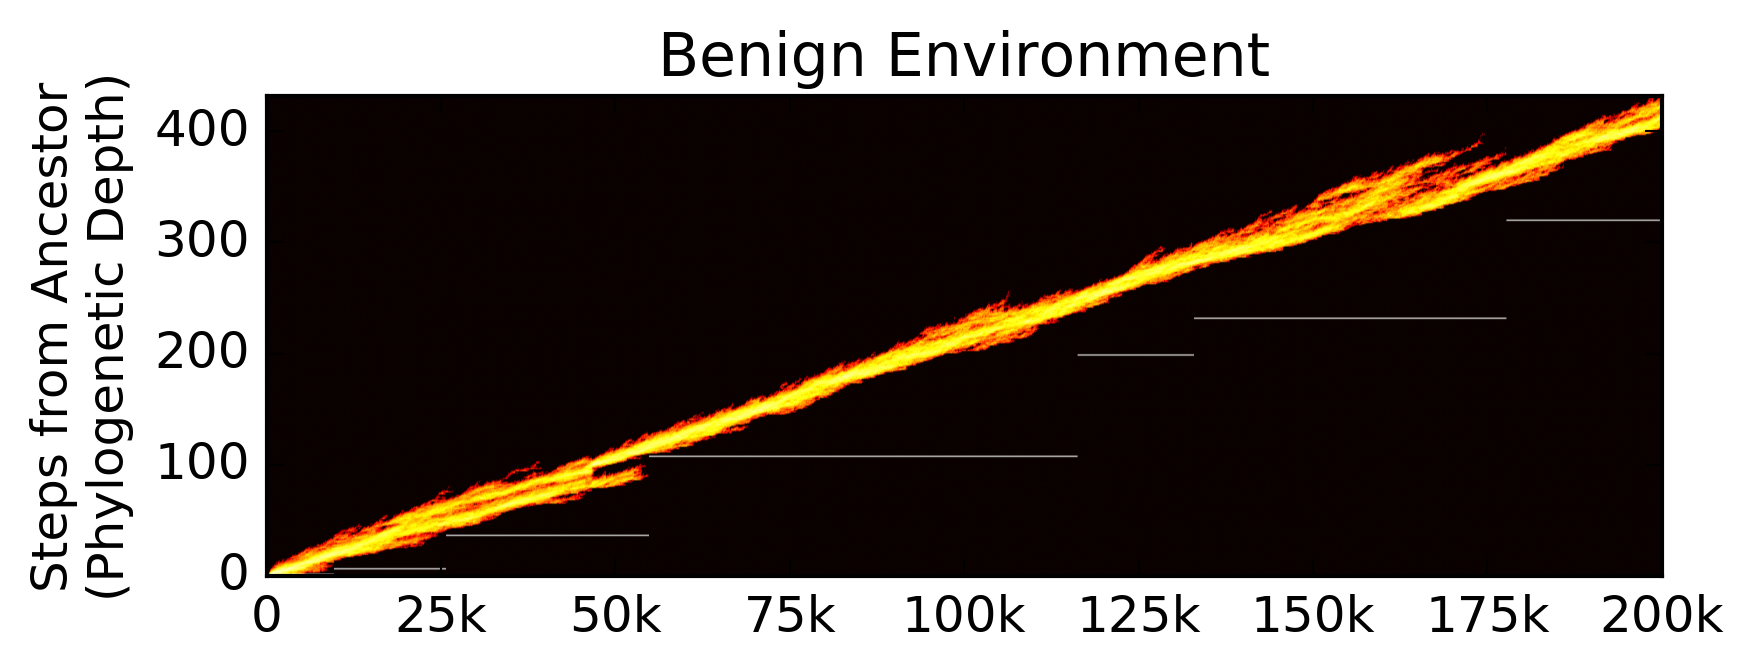
\includegraphics[trim={0.2cm 0 0.25cm 0},clip,width=1\columnwidth]{figures/benign__phylodepth_with_coalescense.png}
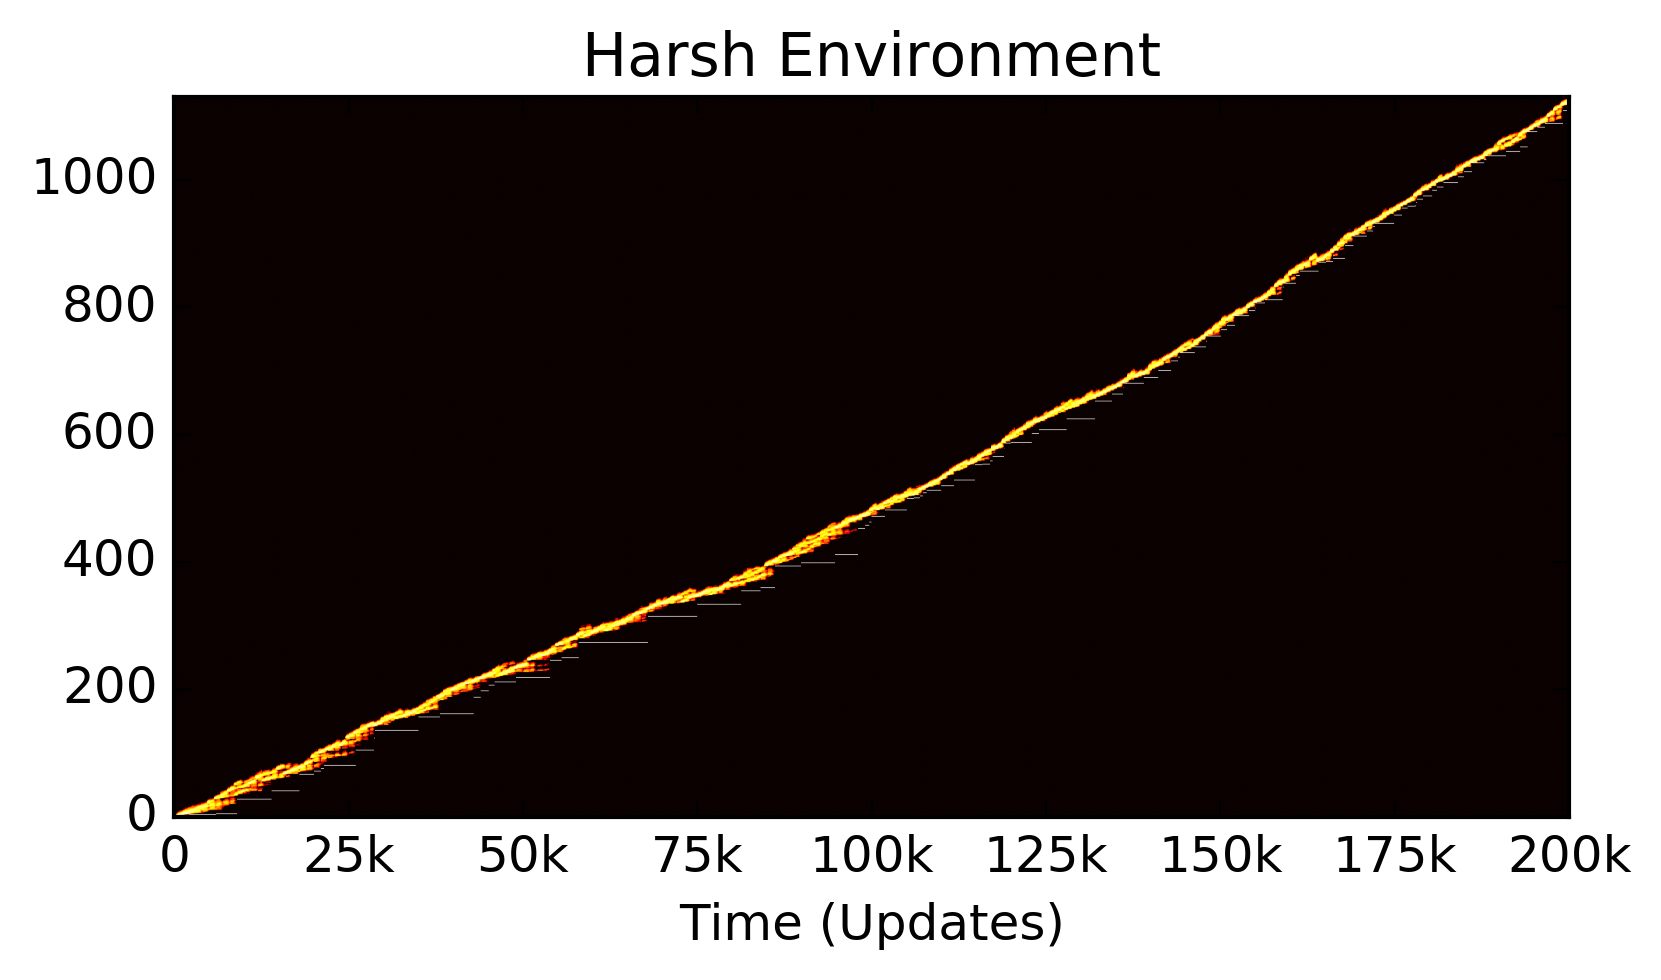
\includegraphics[trim={-0.63cm 0 0.25cm 0},clip,width=1\columnwidth]{figures/harsh__phylodepth_with_coalescense.png}
\caption{{\bf Phylogenetic depth over time of a representative sample population} evolved in each of the three treatments of the cyclic changing environments. White horizontal lines mark the depth of the most recent common ancestor, and discontinuities in this line indicate that the most recent common ancestor has changed, and thus that a sweep occurred. The control treatments had a mean of 18 sweeps (STD=9.05), the benign treatments had a mean of 21 (STD=19.05), and the harsh treatments had a mean of 88 sweeps (STD=23.37). Note the difference in scales between y-axes: the control-evolved population has a maximum depth of 400 mutational steps from ancestor, while the harsh-evolved has upward of 1100. %
}\label{fig:flamegraph}
\end{figure}

%=more genetic diversity
The populations that evolved in the control and benign environments displayed more genetic diversity as compared to those evolved in the harsh cyclic environment, which underwent a bottleneck at each cycle shift. Because a selective sweep reduces current diversity within a population, the smaller number of sweeps
% @CAO it looks like it wasn't just a smaller number of sweeps, but that the sweeps took MUCH longer to occur, to the point where it's hard to even dub them sweeps at all...  more fixation events?  Mike should weigh in here too.
in the benign and control treatments led populations in them to have higher standing diversity for most of their evolutionary history than those populations from the harsh changing environment.  Despite this higher standing diversity in the benign and control treatments, regions of low diversity are still evident in the genomes of these populations, implying purifying selection on the traits encoded at these sites (see Fig~\ref{fig:entropy}).
% * <mjwiser@gmail.com> 2017-01-30T19:39:00.542Z:
%
% I feel like this figure would be easier to talk about if you split it into three panels, and mention that each panel has both an upper and a lower part.  It would also probably be easier to read if the axes on the left were on the top panel, rather than the middle one; since you have two graphs in each panel, it doesn't make sense to just have a single axis label off to the side.  However, you probably *can* have only a single x axis label, since the axes are the same for all the panels, and for both graphs within a panel.
%
% ^.
%@RCK - TODO fix figure below.

%=[FIGURE - entropy][TODO - tidy up this figure]
\begin{figure}[!h]
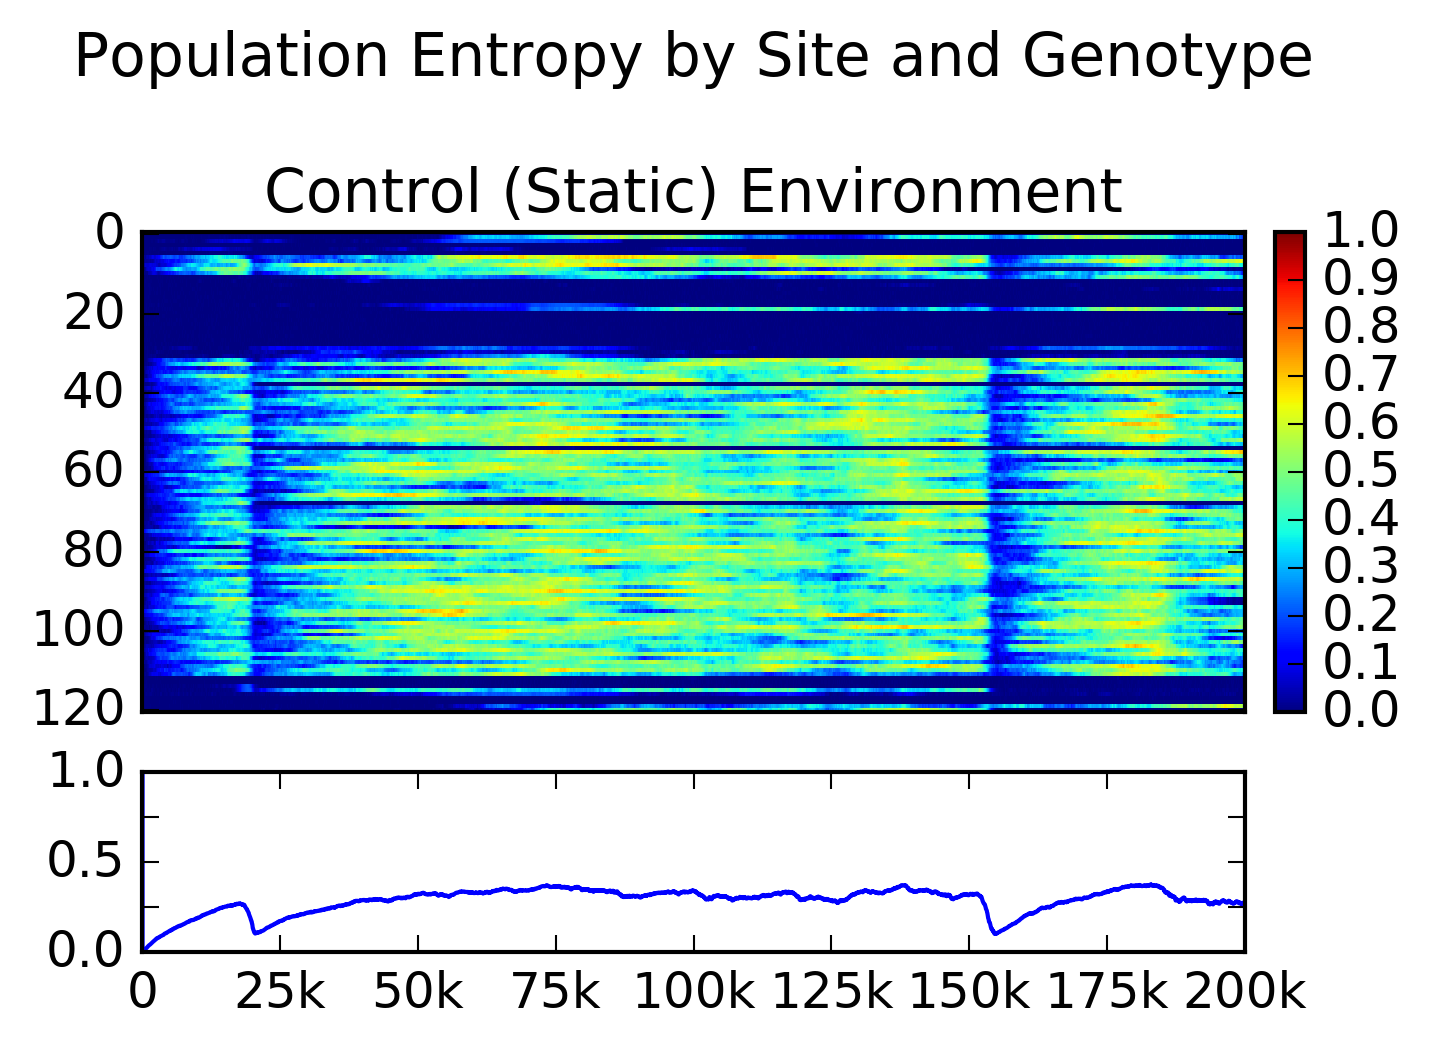
\includegraphics[trim={-0.85cm 0 0.1cm 0.2cm},clip,width=1\columnwidth]{figures/control__entropy}
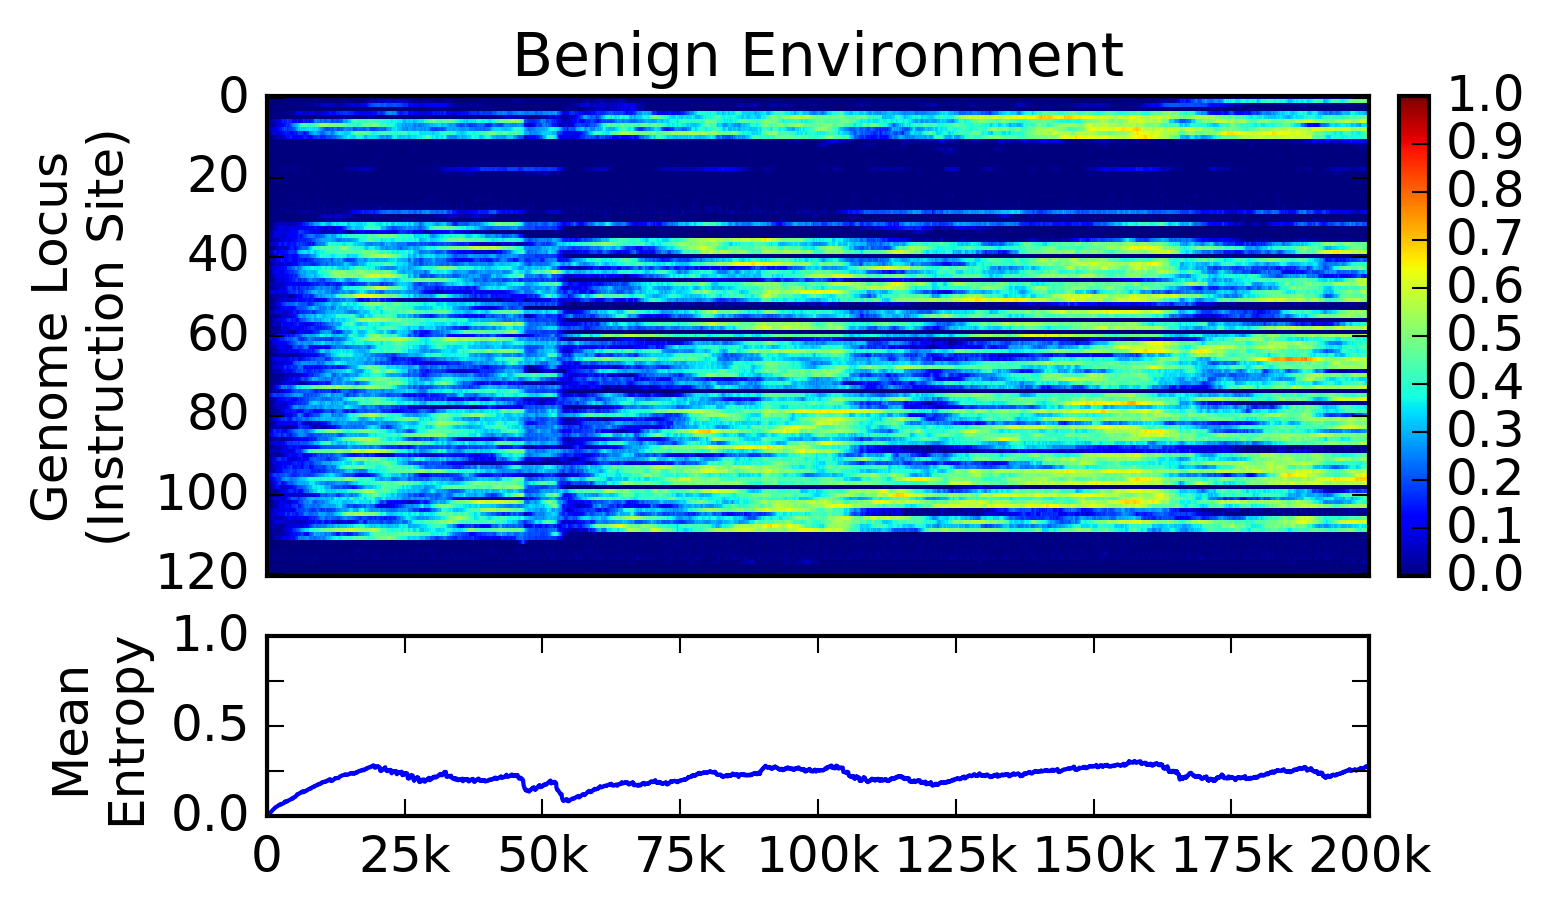
\includegraphics[trim={0.25cm 0 0.1cm 0},clip,width=1\columnwidth]{figures/benign__entropy}
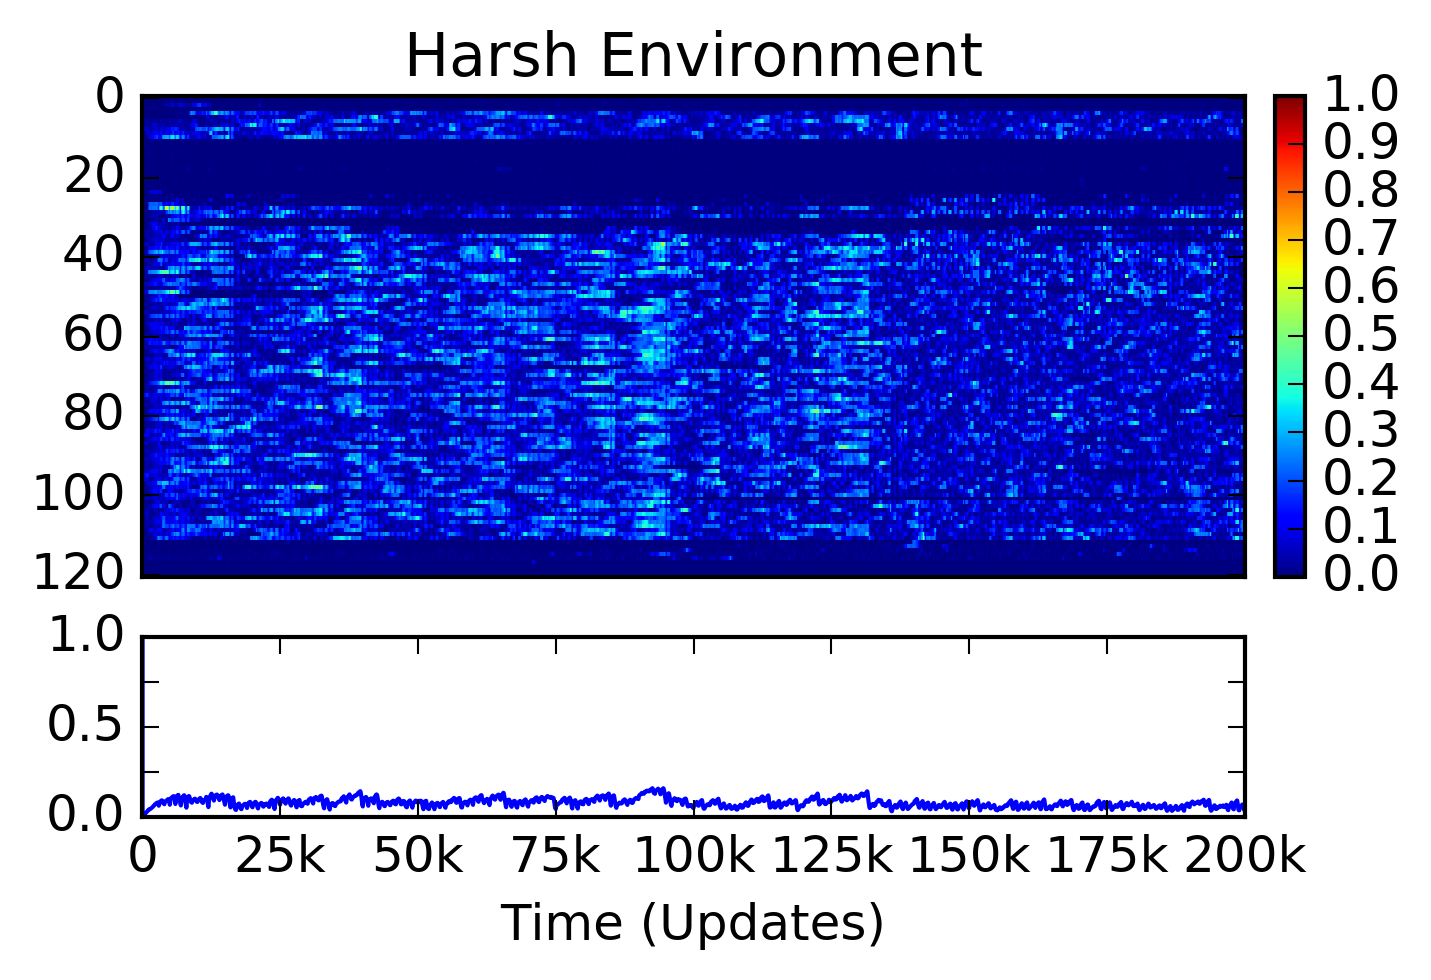
\includegraphics[trim={-0.85cm 0 0.1cm 0},clip,width=1\columnwidth]{figures/harsh__entropy}
\caption{{\bf Population Per-site Entropy over time} of a representative sample population. Each vertical slice represents the per-site entropy of the population at each update, both by genetic locus (upper), and overall population mean (lower). Hotter colors (red/orange/yellow) indicate greater diversity at this locus, while cooler colors (blues) indicate the a locus is more consistent across the population. Mean population entropy indicates the relative diversity of the population at any given time, while the per-site entropy shows where in the genomes the population diversity is located.   %@CAO: I'm agreeing with Mike that we might want to make this two graphs.  I added a bit in the description about the cooler colors just to lead the reader by the hand as much as possible.
}\label{fig:entropy}
\end{figure}


\subsubsection*{Genetic Architecture}
%=genetic architecture is different in benign and harsh vs control
The selective shifts in both benign and harsh changing environments result in qualitatively different architectural styles from the static control environment. The task arrangements evolved under both experimental treatments are much more scattered throughout the genome than in the control. Specifically, the bulk of the sites responsible for performing the fluctuating task (EQU) did not overlap with the backbone task (XOR), except for a core region, which represents portions of the tasks that are shared between XOR and EQU. (Fig~\ref{fig:lineage})
% @CAO: I'm not positive I understand this description for how things are laid out.  It might be worth putting a bit more detail here, and highlighting also that there is a lot more separation in the harsh environment (or so it seems).  Should we talk more here about why all of this is the case (highlighting that we are speculating) or will that come later?

%=[FIGURE - task layout][TODO - polish this figure]
\begin{figure}[!h]
\setlength{\fboxsep}{0pt}%
\setlength{\fboxrule}{0pt}%
\fbox{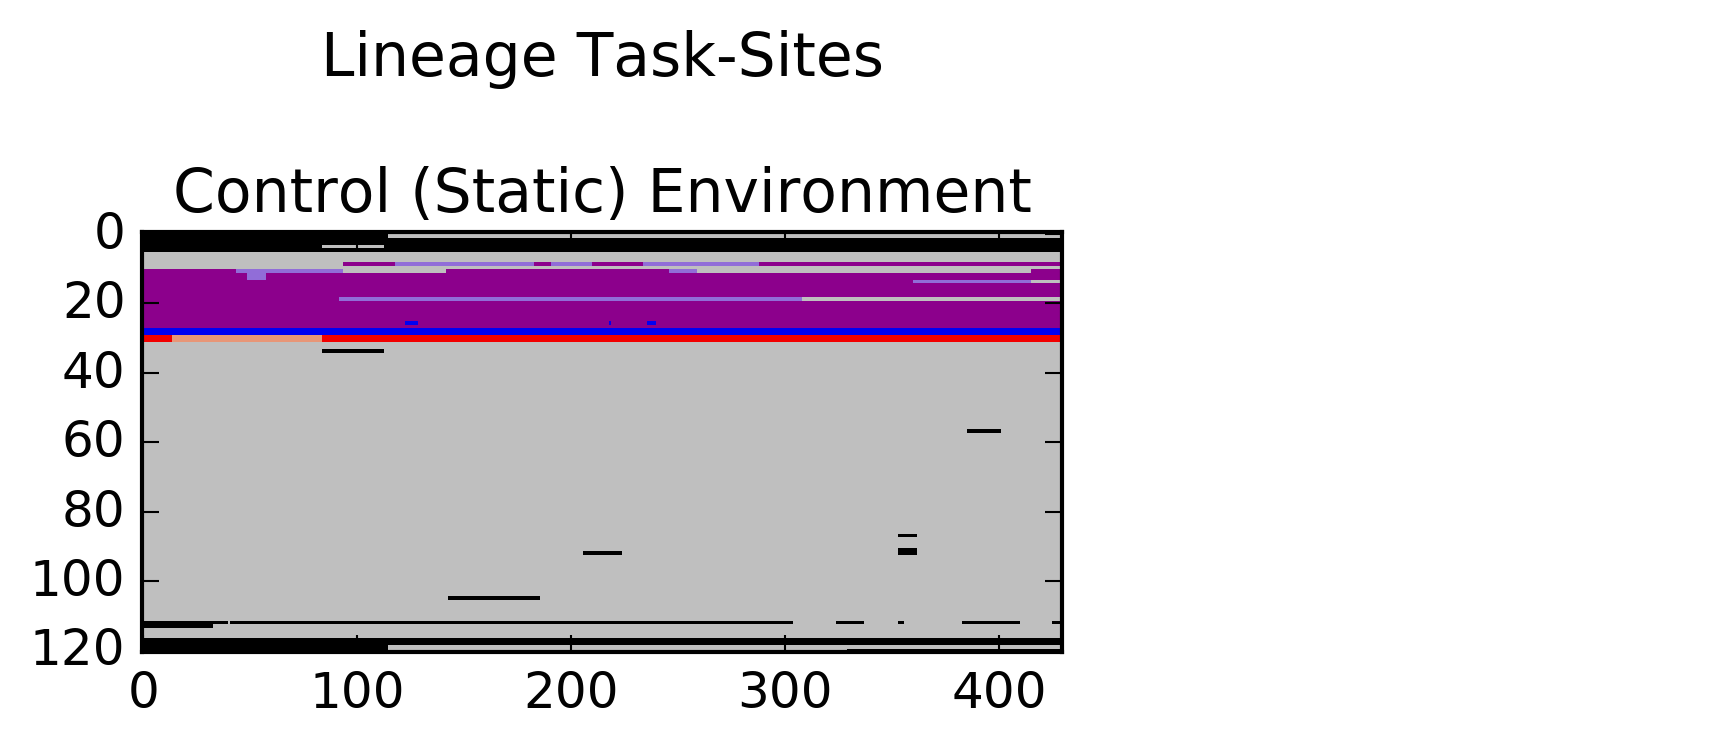
\includegraphics[width=0.75\columnwidth,trim={-0.82cm 0 5.5cm 0.25cm},clip]{figures/control__whole_taskmap.png}}\fbox{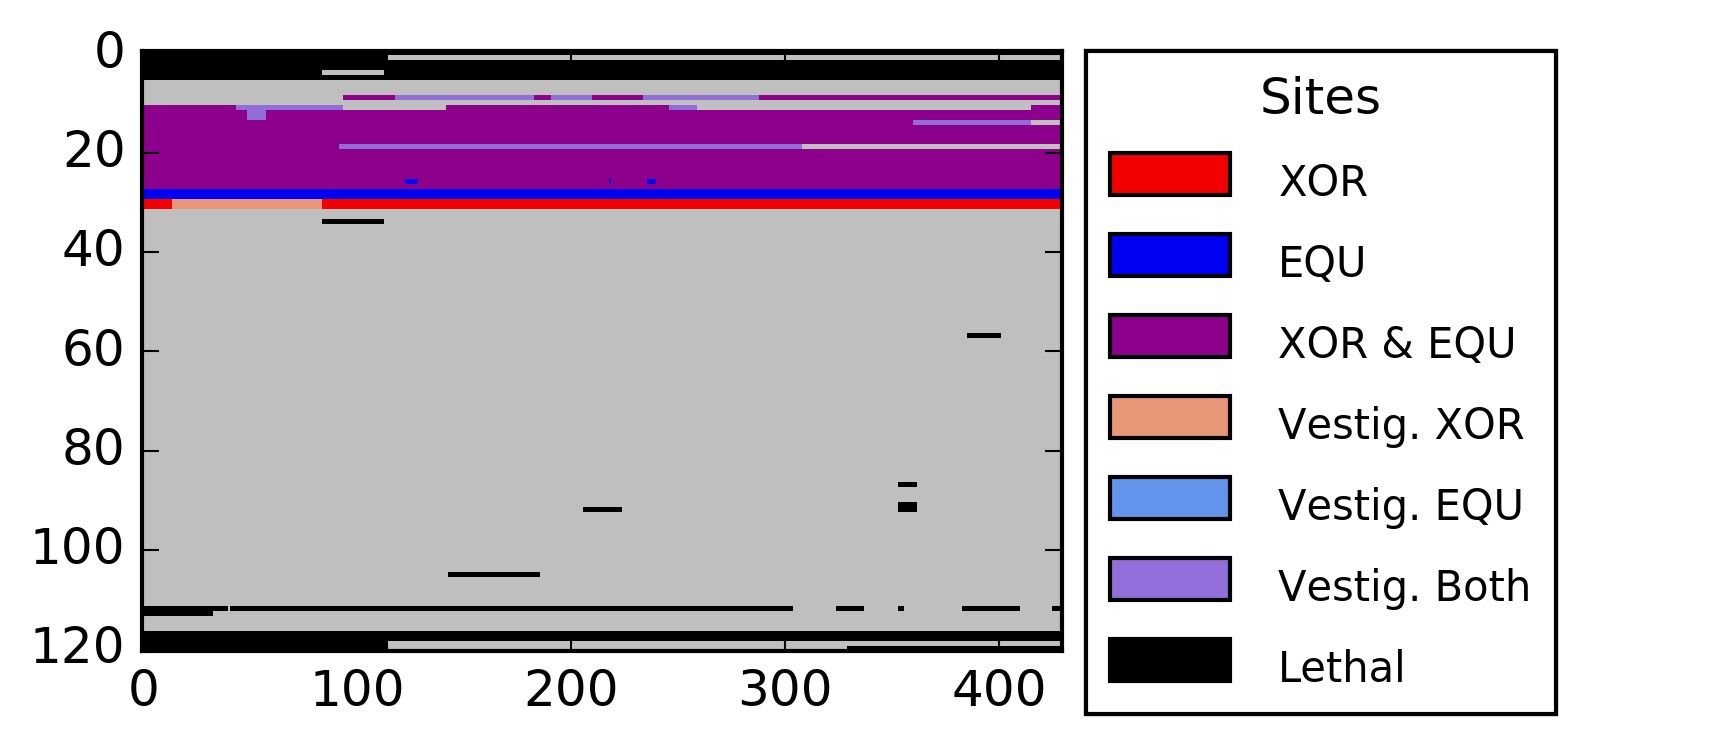
\includegraphics[width=0.25\columnwidth,trim={9.1cm 0.15cm 1.3cm 0},clip]{figures/legend__whole_taskmap.png}}
\fbox{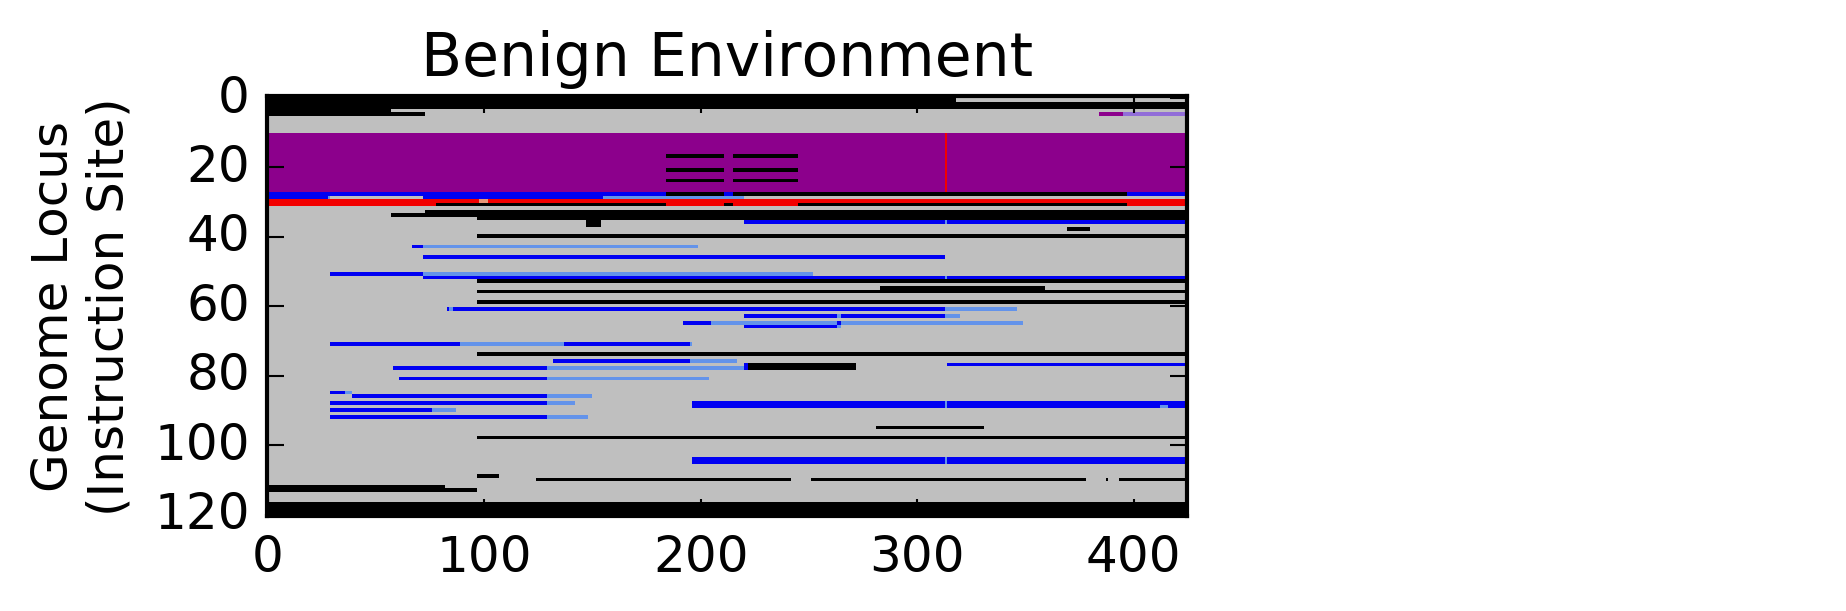
\includegraphics[width=1\columnwidth,trim={0.2cm 0 2.3cm 0},clip]{figures/benign__whole_taskmap.png}}
\fbox{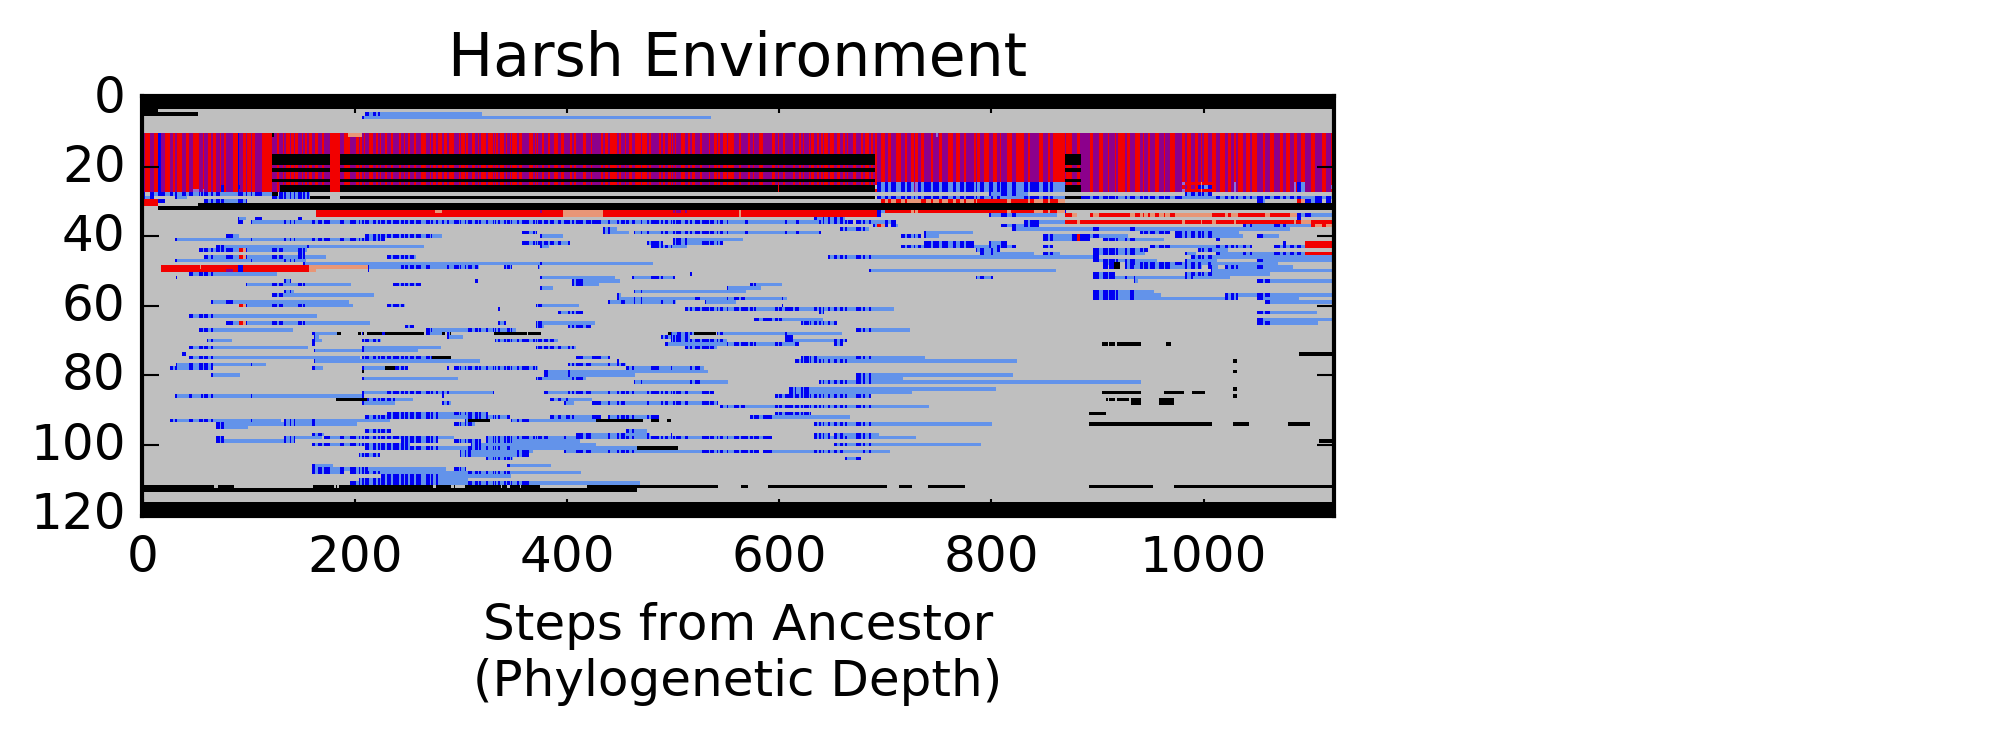
\includegraphics[width=1\columnwidth,trim={-0.82cm 0 5.2cm 0},clip]{figures/harsh__whole_taskmap.png}}
\caption{{\bf Varying genetic architecture of XOR and EQU over time} for the final dominant genotype in a randomly selected replicate. Proceeding from the left of each figure, each vertical slice represents an organism along the line-of-descent to the final dominant.
Positions along the Y-axis represent each genome locus; loci in an organism are colored based on the tasks that they code for. Sites in \textbf{red} are active sites that code for the XOR task only, sites in \textbf{blue} are active sites for the EQU task only, and \textbf{purple} sites code for both XOR and EQU. Knockouts to the sites in black are lethal to the organism. Sites in the lighter colors (tan, light blue, lavender) represent vestigial sites for XOR only, EQU only, or both tasks, respectively. As we proceed from left to right, we can see the evolutionary history of the final dominant genotype.}
\label{fig:lineage}
\end{figure}

%=arch of control, scattered XOR
In contrast, the architecture of XOR and EQU remain tightly intertwined in the control, and site positions do not change substantially over the course of the experiment. In the benign treatment, many more regions that perform the fluctuating task (XOR) are scattered throughout the genome, but site positions remain relatively fixed throughout the run after an initial adaptive phase. In the harsh treatment, not only are the active sites scattered, but the positions of active sites change and proliferate wildly over time.

%=reservoir of vestigial sites
Interestingly, populations evolved in both the benign and harsh treatments also show development of a large reservoir of formerly functional, now vestigial, sites; that is, sites that remain unchanged from when they were previously active in performing a task, but were disabled by a mutation elsewhere and are thus now neutral. These vestigial pseudogene-like sites appear to be important for allowing the organisms to quickly re-adapt as the fluctuations in the environment restore the previously-rewarded functions. (Fig~\ref{fig:CCE_func_vestigial})

%=[FIGURE - functional vs vestigial sites][TODO - stats]
\begin{figure}[!h]
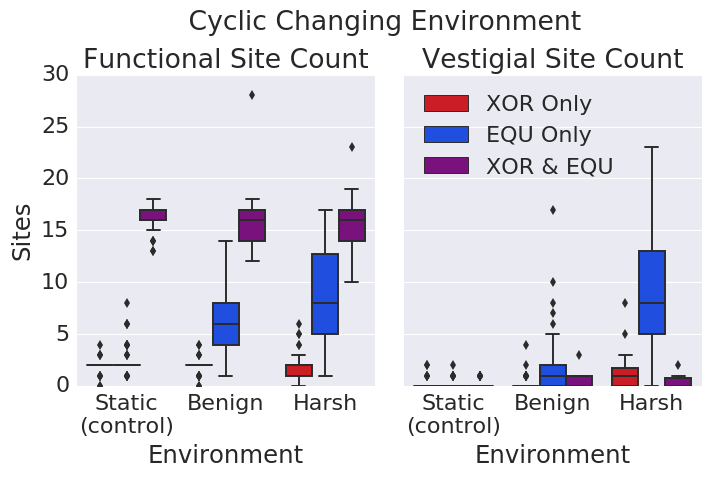
\includegraphics[trim={0 0 0 0}, clip, width=1\columnwidth]{figures/CCE_func_vest__box.png}
%% TODO - generate the stats
\caption{{\bf Number of functional and vestigial sites by treatment}. The harsh environment has a significantly larger number of vestigial sites for the fluctuating (EQU) task compared to the benign treatment or control, while having a comparable number of functional sites (One-Way ANOVA F(X,YYY) = ZZ.ZZ, p $<<$ 0.000QQ).%
%old --- (One-Way ANOVA F(2,132) = 54.35, p $<<$ 0.0001).
% @CAO: Just a reminder to do the stats!
}
\label{fig:CCE_func_vestigial} %% FIGURE 5
\end{figure}

\subsubsection*{Nearby mutational landscape}
%=one-step survey of the mutational landscape [TODO - fix wording to clarify]
In order to identify the role that these pseudogene-like structures play, we performed a survey of the single-step mutational landscape surrounding the most abundant genotype at the end of the experiment for each replicate population. This landscape contained 3,025 distinct mutants (121 loci with 25 possible mutations per locus) in each of the 50 replicates per treatment, for a total of nearly 450,000 mutants surveyed.We found that the availability of reservoirs of vestigial sites shifted the change-evolved organisms' position in the mutational neighborhood, such that a task that was lost due to mutation remains more accessible via one or two additional mutational steps. (Fig~\ref{fig:CCE_single_step}, ~\ref{fig:CCE_two_step})
% @CAO: This last part doesn't make a lot of sense -- CLEARLY if a single mutation causes a task loss, the corresponding reverse mutation would cause that task to be regained.  As such, do you mean that there a MORE paths back to the task in the changing-environment treatments as compared to the static control?
% @RCK: Yes, that's what this means. "More often, above". I can clarify. -- TODO

%=[FIGURE - Frac 1-step][TODO STATS]
\begin{figure}[!h] %% FIGURE 6
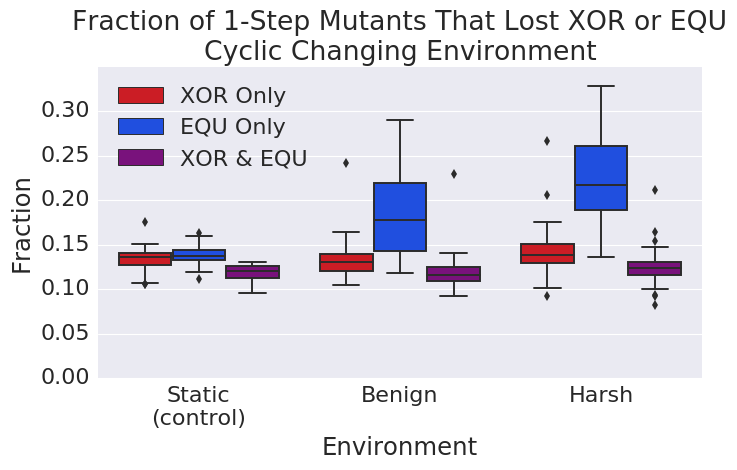
\includegraphics[trim={0.2cm 0 0 0.2cm},clip,width=1\columnwidth]{figures/CCE_frac_1step__box.png}
%% TODO - stats
\caption{{\bf A survey of the single-step mutational neighborhood} around organisms that performed the fluctuating task. Note that in both the benign and harsh treatments, there were significantly more mutants that lost the EQU task as compared to the control (Wilcoxon Rank Sum Test: Z = X.XX and Y.YY respectively, p $<<$ 0.000ZZ). This result indicates that it was easier for the organisms in both treatments to turn off the EQU task in response to one mutation. %
% old -- (Wilcoxon Rank Sum Test: Z = -6.59 and -6.70 respectively, p $<<$ 0.0001)
}\label{fig:CCE_single_step}

\end{figure}
%=[FIGURE - Frac 2-step][TODO STATS]
\begin{figure}[!h] %% FIGURE 7
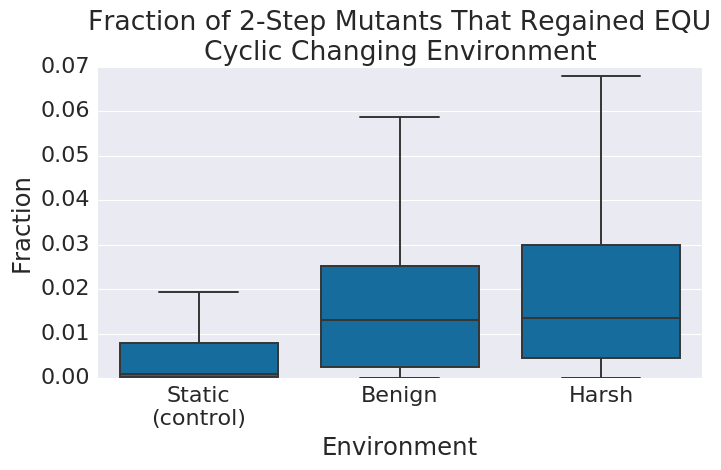
\includegraphics[trim={0.2cm 0 0.4cm 0.25cm},clip,width=1\columnwidth]{figures/CCE_frac_2step__box.png}
%TODO - stats
\caption{{\bf A survey of the two-step mutational neighborhood} of the organisms that lost EQU function in the one-step survey. We found that in both the harsh and benign treatments, there were significantly more organisms that regained function in response to mutation than the control. (Wilcoxon Rank Sum Test: Z = X.XX and Y.YY respectively, p $<<$ 0.000Z). This result indicates that it was easier for the organisms in both fluctuating environments to regain the task in response to one additional mutation.
%(Wilcoxon Rank Sum Test: Z = -6.11 and -7.38 respectively, p $<<$ 0.0001)
}\label{fig:CCE_two_step}
\end{figure}

%=measured D_g, D_p, found similarity in D_g, increase in D_p 
We also measured the proportion of non-deleterious mutants in the nearby fitness landscape. We found that between all treatments, this proportion
remained approximately the same. However, we found that the proportion of these mutants with different (potentially adaptive) phenotypes increased in the changing environments. In this way, the organisms from the changing environment treatments have an advantage over organisms from the control runs in terms of the short-term evolvability of the fluctuating task. This result indicates real adaptation, not only to resources in their local environment, but a direct adaptation to the environmental change. (Fig~\ref{fig:CCE_diffusion_rate})

%=[TODO - add paragraph describing/speculating about why Benign loses EQU almost as well as Harsh]
% @CAO: I also get why we should expect to see EQU lost easily in the Harsh changing environment, but why is it also lost so easily in the benign environment.  Should we speculate here?  (Or do you below?)  More generally, why do you think this is the case?
% @CAO: One other thought for how this result may happen.  Maybe in the control there is a pressure for EQU to evolve to be more robust, whereas the changing environment just doesn't give it time to evolve robustness.  I can't think of a way to easily disentangle those explanations though...
% @RCK: clarify that benign are lost due to drift.
% @RCK - NOTE TO SELF -- see about joining vestigial sites paper with Matt's bias work. Are vestigial sites useful because they are random building blocks available (equivalent to mutational bias), or is there a deeper functional structure. Does order matter?

%=[FIGURE D_g D_p][TODO STATS]
\begin{figure}[!h] %% FIGURE 8
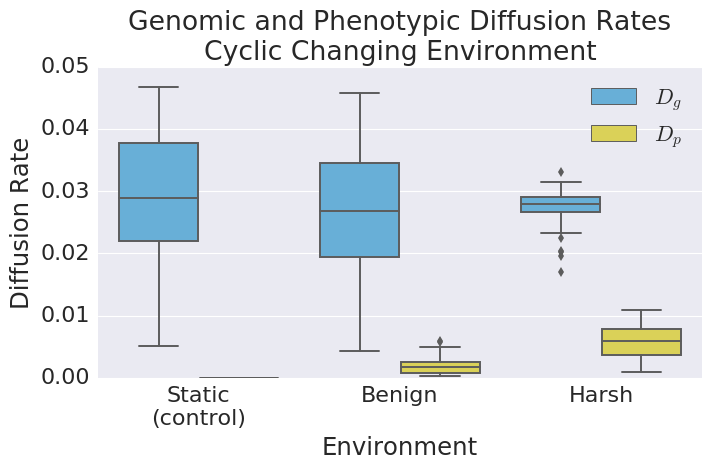
\includegraphics[trim={0.2cm 0 0.4cm 0.25cm},clip,width=1\columnwidth]{figures/CCE_D_g_D_p__box.png}
% TODO -- stats
\caption{{\bf Genomic and Phenotypic Diffusion Rates}, showing the probabilities of producing offspring that are genotypically ($D_g$) or phenotypically ($D_p$) distinct from the parent, while not reducing fitness.
Note that while overall neutral exploration capacity remains relatively stable between treatments, phenotypic exploration capacity is increased in both treatments, but especially in the Harsh treatment. (Wilcoxon Rank Sum Test: Z = XX and XX respectively, p $<<$ 0.0001). This result indicates that changing environments promote the phenotypic evolvability of populations in particular.
}\label{fig:CCE_diffusion_rate}
\end{figure}




\subsection*{Stochastic Changing Environments}
%= contrary to expectations, SCE weren't better at evolvability (D_g/p)
%=[TODO STATS for drop in SCE-Harsh D_p]
%=[TODO REWORD BELOW]
Contrary to our expectations, stochastic changing environments were no more effective at promoting evolvability than cyclically changing environments. In all measures of evolvability, the stochastic treatments performed similarly to the cyclically changing environments. There was a significant reduction [TODO STATS] in the Phenotypic Diffusion Rate ($D_P$) between the cyclic and stochastic harsh changing environments. Overall, $D_P$ showed much larger variances, but settled on a lower mean in the stochastic harsh treatment as compared to the cyclic harsh, indicating a much lower probability of the population producing offspring that would switch phenotypes neutrally. (Fig~\ref{fig:CSE_diffusion_rate})

%=[FIGURE - D_g/p]
%=[TODO STATS]
\begin{figure}[!h] %% FIGURE 12
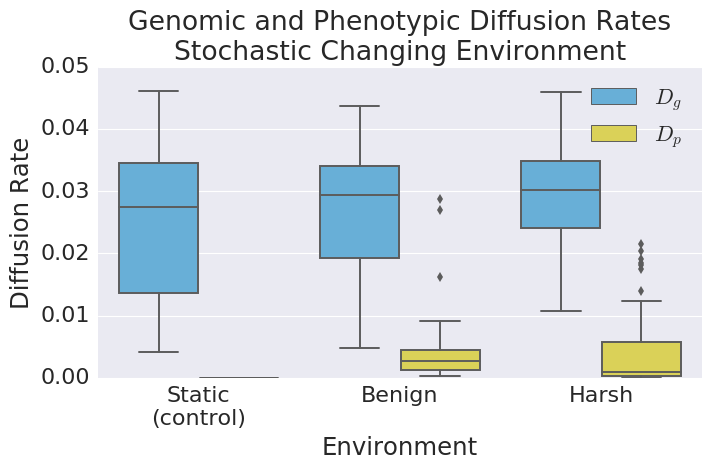
\includegraphics[trim={0.2cm 0 0.4cm 0.25cm},clip,width=1\columnwidth]{figures/CSE_D_g_D_p__box.png}
\caption{{\bf Genomic and Phenotypic Diffusion Rates} in stochastic changing environments, showing the probabilities of producing offspring that are genotypically and phenotypically different from the parent, while remaining fitness neutral or better. As in the cyclic environment $D_g$ remains stable, at comparable levels (TODO STATS), however, the mean is significantly lower (TODO STATS). This result shows that stochastic environments are not as effective as cyclic environments at increasing the probability that organisms will produce phenotypically different, yet neutral offspring.
}\label{fig:CSE_diffusion_rate}
\end{figure}

%=1 and 2-step, slightly reduced
Similarly, both the overall fraction of 1-step mutants that lost EQU, and the fraction of 2nd-step regaining of EQU, were slightly reduced in comparison to the cyclic treatments. This result indicates that stochastic harsh environment was slightly less effective at promoting evolution toward areas of the mutational landscape where such mutations were common.
(Fig~\ref{fig:CSE_single_step},~\ref{fig:CSE_two_step})

%=[FIGURES - 1 & 2-step]
%=[TODO STATS]
\begin{figure}[!h] %% FIGURE 10
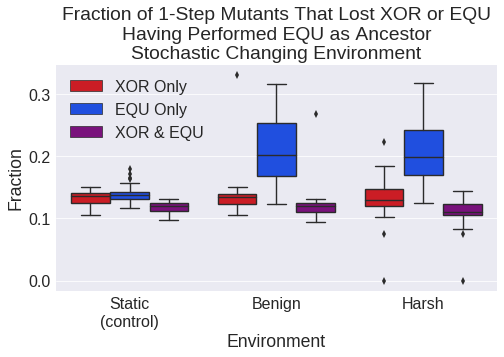
\includegraphics[trim={0.2cm 0 0 0.2cm},clip,width=1\columnwidth]{figures/CSE_frac_1step__filtered__box.png}
\caption{{\bf A survey of the single-step mutational neighborhood} in the stochastic changing environment around organisms that performed the fluctuating task. Again, in the static and benign treatments, values are comparable to the cyclic changing environment (TODO STATS). However, in the harsh treatment, the means for both loss of the fluctuating task (EQU) and loss of both task were slight reduced. (TODO STATS). This result indicates that in the context of a harsh treatment, stochastic environmental change is less effective at moving organisms to areas of the fitness landscape where they can more easily switch task expression. %
}\label{fig:CSE_single_step}
\end{figure}
\begin{figure}[!h] %% FIGURE 11
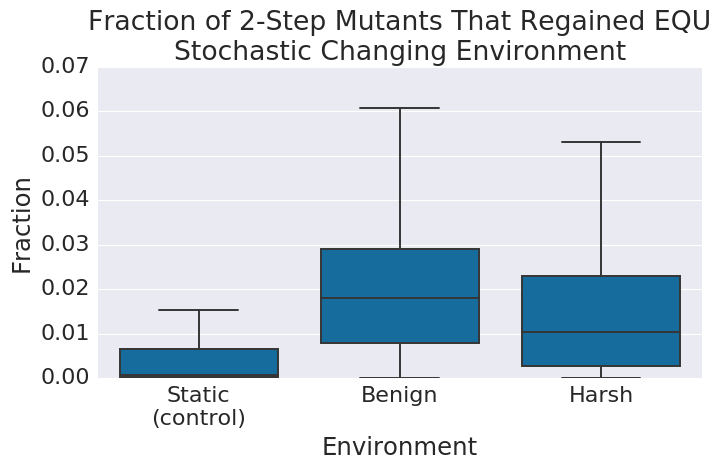
\includegraphics[trim={0.2cm 0 0.4cm 0.25cm},clip,width=1\columnwidth]{figures/CSE_frac_2step__box.png}
\caption{{\bf A survey of the two-step mutational neighborhood} in the stochastic changing environment of the organisms that lost EQU function in the one-step survey. Similarly to the result in Fig~\ref{fig:CSE_single_step}, we found that the fraction of organisms regaining the fluctuating task from a single additional mutation in the harsh treatment were reduced compared to the cyclic harsh treatment. (TODO STATS). This result confirms that the harsh stochastic environment is less effective than the cyclic harsh at promoting evolvability.
}\label{fig:CSE_two_step}
\end{figure}

%=discussion of function vs vestigial
%=[TODO STATS]
The greatest differences between the cyclic and stochastic treatments appeared in the number of functional and vestigial sites. While the functional site counts in the stochastic environment were, overall, relatively similar to those in the cyclic environment, the pattern was different for the vestigial sites. In the stochastic harsh treatment in particular, there was a small, but significant reduction in the number of XOR+EQU overlapping functional sites as compared to the cyclic treatment. Further, there was an overall reduction in the number of EQU-only vestigial sites. These features may provide a clue, indicating that architectural features that would promote the retention of EQU were less prevalent in the harsh stochastic environmental treatment. (Fig~\ref{fig:CSE_func_vestigial}) 

%=[FIGURE - func vestigial sites]
%=[TODO STATS]
\begin{figure}[!h]
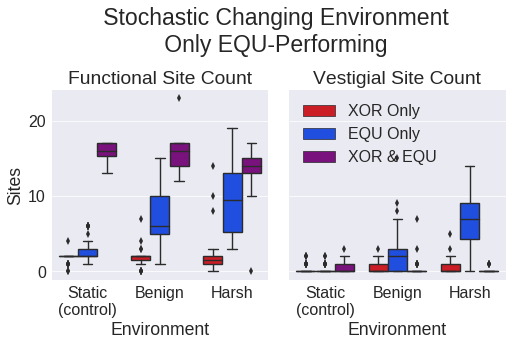
\includegraphics[trim={0 0 0 0}, clip, width=1\columnwidth]{figures/CSE_func_vest__filtered__box.png}
\caption{{\bf Number of functional and vestigial sites by treatment} in a stochastic changing environment. The vestigial site counts remain comparable to the cyclic environment (TODO STATS), however, there was a reduction in functional site counts for XOR+EQU overlapping sites in the stochastic harsh environment as compared to the cyclic harsh environment (TODO STATS), as well as an overall reduction in the number of vestigial sites. (TODO STATS)%
%-old (One-Way ANOVA F(2,132) = 54.35, p $<<$ 0.0001).
}
\label{fig:CSE_func_vestigial} %% FIGURE 9
\end{figure}

%=hypothesyze these effect driven by variance in timespans
%We hypothesize that these effects were driven by the inconsistent time spans between the population experiencing a given environmental condition in the stochastic treatments. Especially long time spans without a reward for a task, even if rare, could allow vestigial sites to drift away, thus pushing subsequent evolution closer to the control treatment. However, due to the rarity of such events, the effects of drift would be relatively limited.
Together, from these measures, we conclude that stochastic environments exert slightly less evolutionary pressure to move toward regions of the mutational landscape that are more congenial to neutral phenotypic exploration and evolvability. We hypothesize that this dynamic may be due to the randomly-occurring environmental changes may either occur too rapidly for a response to selection, or too slowly, such that drift may cause the information contained in vestigial sites to mutate away. While the environment, on average, experiences as many changes as in the cyclic experiment, the distribution of the length of those environment periods may be very different. Thus, we can conclude that our stochastic changing environment is not more effective than a cyclic changing environment, and under harsh conditions, may actually be slightly worse for promoting the evolution of evolvability.

\subsection*{Long-Term Evolvability}

\section*{Conclusion}
In cyclic changing environments, the direction of selection shifts frequently, and periodically drives populations to not only explore new regions of the genetic landscape, but also to carry with them vestigial genetic information about previous environmental conditions. Thus, the resulting populations are not only adapted to the current environment, but also to the meta-environment of cyclic change. Because of their evolutionary history, the genomes contain vestigial fragments of genetic material that were adapted to prior environments. As this exploration proceeds, mutations accumulate in the population, each creating a link to a new region of the mutational landscape. As these links accumulate, they form a reservoir of mobility for the population to quickly shift to new phenotypes as dictated by current selective conditions. In this way, the accumulation of vestigial or pseudogene-like regions acts as an adaptation to the larger pattern of changing selective forces.

By contrast, in static (non-changing) environments, the majority of neutral mutations do not connect to as many phenotypically-interesting regions of genotype-space. There are far fewer pseudogene-like regions available that could regain functionality should conditions change. Thus, populations evolved in static environments are less evolvable in the short-term.

Surprisingly, stochastically changing environments were slightly less effective at exploration
% @CAO: Are they really?  We've shown that they produce new phenotypes less often, but that's a very limited definition of exploration.  However, it's the one that we need to stick to.
% @CAO: That said (and this argument goes to static environments too), if we claim that stochastic environments produce new phenotypes less frequently we can argue WHY we hypothesize that they'll be less effective at exploration.  In thinking about it, it feels like we should use these as ancestors for an entirely new environmental shift.  If we show that the organisms previously experiencing a cyclically changing environment do better with the new environment THEN we have strong evidence that stochastically changing environments are less effective at exploration.
than cyclic changing environments, even if, on average, the amount of time spent in each environment was equal. We hypothesize this is because of more opportunity for drift to destroy the information contained in vestigial regions, as well as potentially fewer opportunities for populations to respond to selection.

\subsection*{Limitations of Changing Environments}
Changing environments produce a set of selective pressures that speed up exploration of genotype space, while also building reservoirs of partial functionality that may be co-opted in the evolution of more complex structures. These features make changing environments useful for both their explanatory power in natural evolution, and as practical tools in the Artificial Life toolkit.
Ultimately, however, cyclic changing environments only re-tread existing phenotypic ground, and though genotypic exploration is faster than under purely directional or stabilizing selection, the space explored remains constrained by the type of phenotypes that are selected.

Even so, there must exist methods of exploring genotype space that do not suffer from these limitations.
For example, perhaps repeated bottlenecking of populations could promote faster traversal of the fitness landscape in quasi-random directions.
More ambitiously, perhaps these kinds of environments could be coupled with dynamically increasing open-ended complexity goals.

%% TODO Tweak below?
Understanding the mechanisms by which select environmental conditions alter fitness landscapes is vital to understanding the forces that promote evolvability and increase complexity. In particular, understanding the role of vestigial sites may help us untangle how robustness can promote evolvability. Are these vestigial sites inactive remnants, reservoirs of function, or are they part of a complex compensatory framework supporting and buffering the expression of the phenotype? Or both? Changing environments provide one view into these dynamics, but we must explore further to find other mechanisms for exploring and exploiting genotype space.

\section*{Acknowledgments}
We would like to thank Alex Lalejini for helpful discussions and comments about the relationship between phenotypic plasticity and contingency loci, Josh Nahum for discussions of experiments in changing environments, and Emily Dolson, Brian Goldman, and Anya Vostinar for their comments on early manuscript drafts.
This material is based in part upon work supported by the National Science Foundation under Cooperative Agreement No. DBI-0939454 to CO and a Graduate Research Fellowship to RCK. Any opinions, findings, and conclusions or recommendations expressed in this material are those of the author(s) and do not necessarily reflect the views of the National Science Foundation.

%\bibliographystyle{apalike}
\bibliography{changing_env}



\end{document}